%TODO switch and add empty pages at the beginning and remove at the end
%\documentclass[12pt,a4paper,twoside]{article}
\documentclass[12pt,a4paper]{article} % hidelinks
\usepackage[utf8]{inputenc}
\usepackage{amsmath}
\usepackage{amsfonts}
\usepackage{amssymb}
\usepackage{amsthm}
\usepackage{makeidx}
\usepackage[english]{babel}
\usepackage{graphicx}
\usepackage{wrapfig}
\usepackage{lipsum}
\usepackage{physics}
\usepackage{tabularx}
\usepackage[usenames, dvipsnames]{color}
\usepackage{multirow}
\usepackage{array}
\usepackage{float}
\usepackage{caption} % For linebreaks in captions
\usepackage[per-mode=fraction, binary-units=true]{siunitx}
\usepackage[onehalfspacing]{setspace}
%TODO switch
%\usepackage[left=2.5cm,right=3.5cm,top=3cm,bottom=3cm, twoside]{geometry} 
\usepackage[left=3cm,right=3cm,top=3cm,bottom=3cm]{geometry}

\setlength{\parindent}{0in} 

\newenvironment {Zitat}{\par\bigskip \begingroup \leftskip=1cm \begin{itshape} }{\end{itshape} \par\bigskip \endgroup}


% For pseudo assembly code (to explain dependencies) Orange
\newenvironment {assembly}{\begingroup \ttfamily \color{Gray} \begin{itemize} \item[]}{\end{itemize}\endgroup}

% For pseudo high level code
\newenvironment {highcode}{\begingroup \ttfamily \color{Magenta} \begin{itemize} \item[]}{\end{itemize}\endgroup}


\newcommand{\note}{\textcolor{WildStrawberry}}
\newcommand{\greyout}{\textcolor{Gray}}

\newcommand\tab[1][1cm]{\hspace*{#1}}

\newcolumntype{Z}{>{\centering\let\newline\\\arraybackslash\hspace{0pt}}X}


\newcolumntype{a}{>{\hsize = 1cm}X}
\newcolumntype{n}{>{\hsize = .4cm}X} %number
\newcolumntype{o}{>{\hsize = .75cm}X} %opcode
\newcolumntype{R}{>{\raggedleft\arraybackslash}X}
\newcolumntype{C}{>{\centering\arraybackslash}X}

\usepackage{hyperref}
\hypersetup{%
	colorlinks	= false,
	urlbordercolor   = 0.118 0.345 0.608, %RGB values from 0 to 1
	linkbordercolor	 = 0.118 0.345 0.608,
	citebordercolor  = 0.118 0.345 0.608
	%hidelinks   = true
	%frenchlinks = true SMALLCAPS TOC
}

\hyphenation{Pro-zess-or-takt-fre-quen-zen}
\hyphenation{voltage}

\pdfcompresslevel=0			%TODO remove later
\pdfobjcompresslevel=0		%TODO remove later

\renewcommand{\footnoterule}{\rule{0 cm}{0 cm}}
%\renewcommand{\figurename}{Abb.}

\begin{document}
\thispagestyle{empty}
\begin{titlepage}
	\begin{center}
		
		\Large\textbf{Department of Physics and Astronomy\\
			University of Heidelberg}
		
		\vspace{17cm}
		
		\normalsize
		Bachelor Thesis in Physics\\
		submitted by\\
		\vspace{0.5cm}
		\Large\textbf{AMANDA MATTHES}\\
		\normalsize
		\vspace{0.5cm}
		born in Hamburg (Germany) in 1998\\
		\vspace{0.5cm}
		\Large\textbf{2019}
		\normalsize
		
		\newpage
		\thispagestyle{empty}
		
		
		
		
		{\fontsize{21}{30}\selectfont 
			\textbf{Exploiting Instruction-Level Parallelism}
			\par
		}
		\vspace{.5cm}
		%{\fontsize{15}{20}\selectfont Hardware Structures for a Superscalar Out-of-Order Processor}
		{\fontsize{22}{23}\selectfont 
			Hardware Structures\\
			for a \\
			Superscalar Out-of-Order Processor
			\par
		}
		
		\vspace{16cm}
		
		\normalsize
		This Bachelor Thesis has been carried out by Amanda Matthes at the\\
		Institute of Computer Engineering (ZITI) in Heidelberg\\
		under the supervision of\\
		Prof. Ulrich Brüning
		
		\vfill
	\end{center}
	
\end{titlepage}
\newpage 

\pagenumbering{Roman}

\begin{abstract}
	\noindent Superscalar out-of-order execution has become the norm in modern processors. Yet there is little information in the literature about its implementation details. This thesis explores what new hardware structures superscalar out-of-order execution requires. It presents a design for a simple processor, implemented in SystemVerilog, that uses register renaming, reservation stations and a reorder buffer to dynamically schedule instructions.\\
	
	\noindent The thesis also contains an essay that explains why power limitations have caused processor clock rates to stagnate in the noughties. This resulted in heightened pressure on computer architects to increase instruction throughput per cycle.
	
		
	
\end{abstract}
	\vspace{3cm}
\begin{abstract}
	\noindent Fast alle modernen Prozessoren realisieren dynamische, superskalare out-of-order execution. Trotzdem mangelt es in der Literatur an Information zu den Implementationsdetails dieser Maschinen. Diese Arbeit untersucht welche neuen Hardwarestrukturen notwendig sind um superskalare out-of-order execution zu unterstützen. Das Ergebnis dieser Arbeit ist ein einfacher, in SystemVerilog implementierter Prozessor, der diese Ideen umsetzt.\\
	
	\noindent Diese Arbeit enthält außerdem ein Essay, das erforscht weshalb Prozessortaktfrequenzen um etwa 2005 aufgehört haben zu steigen. Dies legte weiter Druck auf Rechnerarchitekten den Instruktionendurchsatz pro Zyklus zu erhöhen und macht es besonders wichtig diese Optimierungsideen zu studieren.\\
	
\end{abstract}
\newpage

\begin{spacing} {1.1}
\tableofcontents
\end{spacing}
\newpage


\pagenumbering{arabic}
\setcounter{page}{1}
\section{Introduction} \label{sec-intro}
As we are reaching the limits that physics sets on the size and speed of our processor components, it is becoming increasingly important to develop sophisticated computer architectures to improve performance. A major contributor to rising instruction throughput in the last three decades has been the introduction of superscalar out-of-order execution to modern processors \cite[p.~3]{lipastiShen} \cite[p.~2f]{Hennessy}.\\ 
Superscalar processors increase throughput by dynamically arranging instructions to execute several of them in parallel in the same core. Out-of-order processors not only dynamically bundle instructions to be executed together, but they even allow for instructions to happen out of their original program order. This enables instructions to overtake instructions in front of them that would otherwise block the pipeline.\\
That is not a new idea. In fact, the original paper by Robert Tomasulo which first described an algorithm to enable superscalar out-of-order execution was published in 1967 \cite{tomasulo}. It was used in 1966 in the large-scale System/360 Model 91, but it took over two decades for microprocessors to implement these ideas again. Since the 90s, superscalar out-of-order execution has become standard in our processors and enabled (single-core) processor performance to continue rising \cite[p.~2f]{Hennessy}. Unfortunately, the literature is often very vague about the implementation details of these machines. \\
The aim of my thesis project was to understand, design and simulate hardware structures that enable superscalar out-of-order execution. The result was a primitive but functioning processor, implemented in SystemVerilog and loosely based on the RISC-V ISA (see p.~\pageref{sec-assembly}).\\

The following section will explain what superscalar out-of-order execution is and how it affects instruction flow and throughput. Section \ref{sec-design} will present my design and describe in detail how it allows for instructions to be dynamically scheduled. Section \ref{sec-results} will demonstrate the functionality of the design by looking at how it handles test cases. This is followed by a short discussion of the limits of superscalar execution and the dangers that out-of-order execution creates in sections \ref{sec-superscalarLimits} and \ref{sec-oooDangers}. Section \ref{sec-outlook} outlines what work remains to be done to turn this design into a fully functioning processor and what alternative approaches exist.\\
Finally, this thesis also includes an essay (p.~\pageref{sec-physicallimits}) which explains why it is necessary to improve the scheduling of instructions at all if a higher clock frequency could achieve the same effect (better performance) without the extra hardware complexity. 


\newpage
\section{Background}
This section gives a quick overview of the different stages of optimising a pipeline and ends with an explanation of what superscalar out-of-order execution is. This information can be found in any computer architecture textbook (e.g. \cite{lipastiShen}, \cite{Hennessy}, \cite{ProcessorArchitecture}).

\subsection{Sequential scheduling and control dependencies}
\begin{figure}[H]
	\centering
	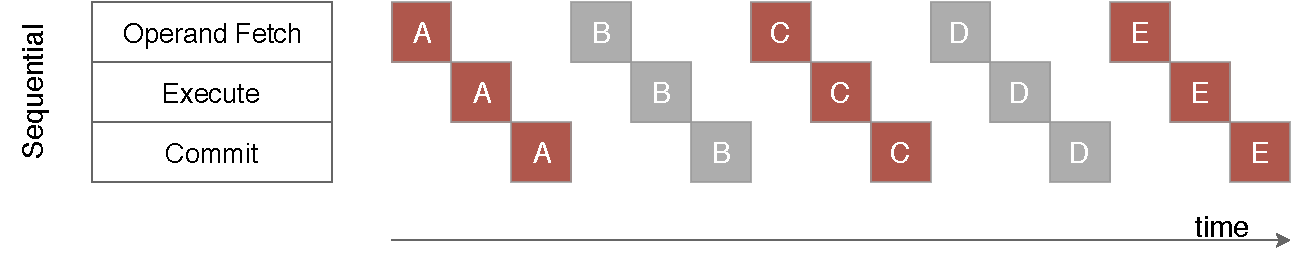
\includegraphics[width=\textwidth]{Source/SchedulingSchemes/Sequential.pdf}
	\caption{Sequential scheduling} 
	\label{fig-sequential}
\end{figure}
In the classic von Neumann architecture, the program counter (PC) always points to the next instruction to be executed. The instruction is fetched from memory, its source operands are fetched, it is sent to the appropriate execution unit, executed and then the result is written back to memory. The PC advances to the next instruction and the same procedure starts again. Usually the PC always increases by one instruction, but jumps and branches can place the PC at any new instruction. Once an instruction is fetched from memory, the three major steps that it goes through are ``operand fetch'', ``execute'' and ``commit''. Figure \ref{fig-sequential} shows how instructions pass through these steps, one after the other. 

\subsection{Pipelining and data dependencies} \label{sec-dependencies}
\begin{figure}[H]
	\centering
	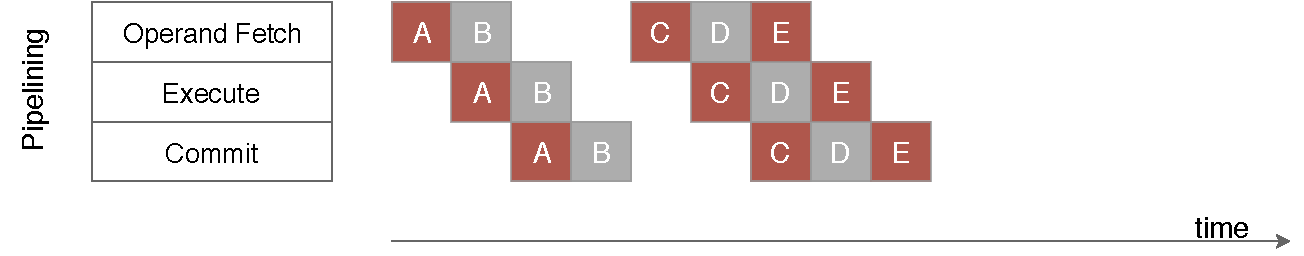
\includegraphics[width=\textwidth]{Source/SchedulingSchemes/Pipelining.pdf}
	\caption{Pipelining} 
	\label{fig-pipelining}
\end{figure}
Different parts of the CPU are responsible for the different stages that an instruction goes through. This means that at any time most of the CPU is doing nothing while it is waiting for the next instruction. The idea behind \textbf{pipelining} is to start the next instruction one clock cycle after the first. Once A has both its source operands and starts execution, B can already start fetching its operands. When A has finished execution, B can start execution and so on. \\
Ideally, each of these steps can be done in one clock cycle. If a processor has a clock frequency of $f=\SI{1}{\GHz} = \SI{e9}{\Hz} $, then one such clock cycle takes $1/f=\SI{e-9}{\second}=\SI{1}{\ns}$.\\ 
The number of \textbf{instructions per cycle} (IPC) that are executed is a measure of throughput. The sequential scheduling scheme above would have an IPC count of $1/d$, where $d$ is the \textbf{depth} of the pipeline, i.e. the number of stages that an instruction has to go through. In our case $d=3$, so our IPC count is $1/3$. In other words, a sequential scheduling scheme completes one instruction every 3 clock cycles. With pipelining, we can achieve an IPC count of \textit{up to one} if the pipeline is perfectly filled and there are no bubbles.\\
Unfortunately, this is not always possible. Consider this code (see p. \pageref{sec-assembly} for how to read this): 
\begin{assembly}
	\begin{tabularx} {\textwidth} {n o a a X}
		1 & LD 	& R1 & 0(R8)	& \\
		2 & LD 	& R2 & 0(R9)	& \\
		3 & ADD & R3 & R1		& R2 \\
	\end{tabularx}
\end{assembly}
The ADD must wait for both LDs to happen before it can use its source operands. This situation is sketched in figure \ref{fig-pipelining} between instructions B and C. The following instructions neatly fill the pipeline but the dependency between B and C creates a stall in the pipeline, a ``bubble''.\\
This is a \textbf{true dependency} or \textbf{flow dependency}. There is no way the ADD can happen before the LDs. Conversely, there are \textbf{false dependencies} or \textbf{name dependencies}, which do not stem from actual data flow. Consider this example, which could be the result of an unrolled loop:
\begin{assembly}
	\begin{tabularx} {\textwidth} {n o a a X}
		1 & LD  & R3 & 18(R1)	& \\
		2 & ADD & R5 & R3		& R2\\
		3 & LD  & R3 & 19(R1)	& \\
		4 & ADD & R6 & R3		& R2\\
	\end{tabularx}
\end{assembly}
There is a true dependency between the first ADD and the first LD, and one between the second ADD and the second LD. However, while instructions \texttt{3} and \texttt{4} are \textit{logically} independent of instructions \texttt{1} and \texttt{2}, they still have to happen strictly in sequence, because of the reuse of R3. This is a false dependency. It limits how much parallelism we can exploit from the code.\\ 
\newpage
Name dependencies can be resolved by \textbf{register renaming}. In our example:
\begin{assembly}
	\begin{tabularx} {\textwidth} {n o a a X}
		1' & LD  & R3 & 18(R1)	& \\
		2' & ADD & R5 & R3		& R2\\
		3' & LD  & \underline{R7} & 19(R1)	& \\
		4' & ADD & R6 & \underline{R7}		& R2\\
	\end{tabularx}
\end{assembly}
The true dependencies between \texttt{1} and \texttt{2} and between \texttt{3} and \texttt{4} remain. But now, there is no reason for the first two instructions to happen before the second two. We could swap them without violating the data flow:
\begin{assembly}
	\begin{tabularx} {\textwidth} {n o a a X}
		3' & LD  & R7 & 19(R1)	& \\
		4' & ADD & R6 & R7		& R2\\
		1' & LD  & R3 & 18(R1)	& \\
		2' & ADD & R5 & R3		& R2\\
	\end{tabularx}
\end{assembly}
We could even imagine them happening in parallel on independent cores:
\begin{figure}[H]
	\centering
	\begin{minipage}{.5\textwidth}
		\begin{assembly}
			\begin{tabularx} {\textwidth} {n o a a X}
				1' & LD  & R3 & 18(R1)	& \\
				2' & ADD & R5 & R3		& R2\\
			\end{tabularx}
		\end{assembly}
	\end{minipage}%
	\vline
	\begin{minipage}{.5\textwidth}
		\begin{assembly}
			\begin{tabularx} {\textwidth} {n o a a X}
				3' & LD  & R7 & 19(R1)	& \\
				4' & ADD & R6 & R7		& R2\\
			\end{tabularx}
		\end{assembly}
	\end{minipage}%
\end{figure}%
This kind of parallelism between instructions that do not depend on each other is known as \textbf{instruction-level parallelism} (ILP). A major goal of CPU design is to find and exploit ILP where possible to speed up a processor without having to increase its clock speed.\\
The difference between true and false dependencies will become very important later when we will try to introduce such parallelism to our execution.

\subsection{Forwarding}
\begin{figure}[H]
	\centering
	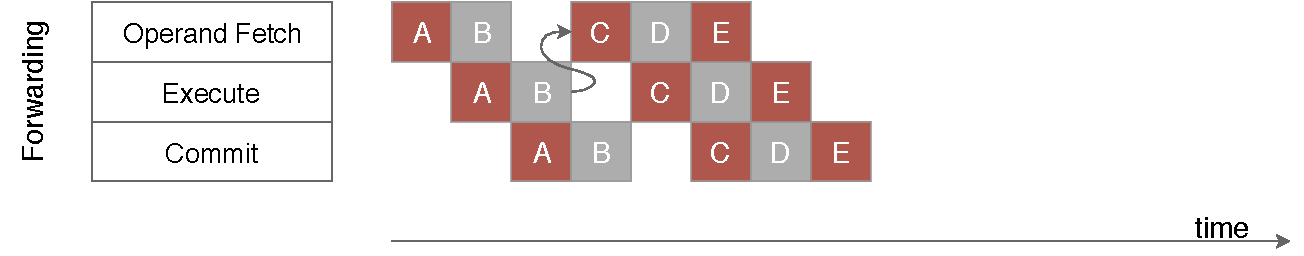
\includegraphics[width=\textwidth]{Source/SchedulingSchemes/Forwarding.pdf}
	\caption{Pipelining with forwarding} 
	\label{fig-forwarding}
\end{figure}
In our example from figure \ref{fig-pipelining} we can see that, with pipelining, instruction C has to wait for instruction B to completely finish, i.e. to commit its result by writing the register file so that B can read it in the next cycle. \\
\textbf{Forwarding paths} in the pipeline allow instruction C to access the result of instruction B once it is calculated rather than having to wait for it to be written to the register file. We can see in figure \ref{fig-forwarding} that this results in slightly tighter scheduling. In that particular example we are not achieving a big speed up, but if we have a piece of code in which many instructions depend on the previous one, forwarding paths can be a major improvement.

\subsection{Superscalar execution}
\begin{figure}[H]
	\centering
	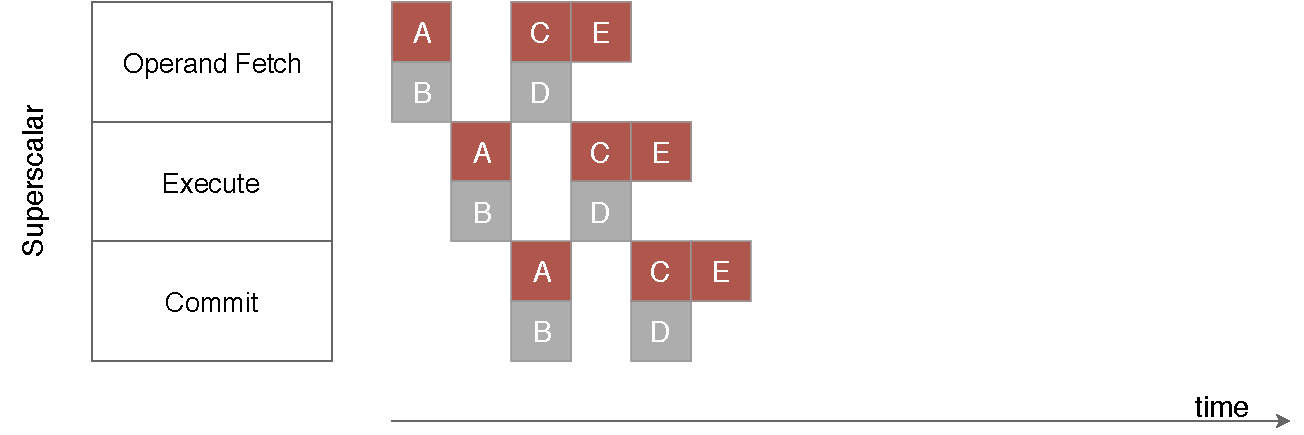
\includegraphics[width=\textwidth]{Source/SchedulingSchemes/Superscalar.pdf}
	\caption{Superscalar execution} 
	\label{fig-superscalar}
\end{figure}
After optimising the IPC count by pipelining in this way, one might wonder if it is possible to optimise any further since all stages of the pipeline are being used whenever possible. However, at any point in time, we are only using one of the execution units. A processor will usually have many of these that specialise in different instruction types. One will be responsible for integer arithmetic, one for loads and stores to the memory, others will specialise in branches, floating point operations or square roots. So we might wonder if it is possible to fill these with other instructions that are ready to be executed. Consider these two instructions:
\begin{assembly}
	\begin{tabularx} {\textwidth} {n o a a X}
		1 & ADD & R3 & R1		& R2 \\
		2 & LD  & R5 & 0(R9)	& \\
	\end{tabularx}
\end{assembly}
They do not depend on each other at all. In hardware, a load instruction will be handled by the load-store unit and an integer addition by the integer unit. We can imagine these two instructions fetching their source operands, executing and committing simultaneously. This is called \textbf{superscalar execution}, as opposed to scalar execution where only one instruction is executed at a time.\\

With superscalar execution, we can reach IPC counts \textit{greater than one}. If we have $w$ execution units that can all work at the same time and all other parts of the processor can handle $w$ instructions at once, then we can reach an IPC count of $w$. We call this the \textbf{width} of the pipeline. In our example (figure \ref{fig-superscalar}) we imagined a pipeline with $w=2$. This maximum is only reached if the pipeline can always be filled. Figure \ref{fig-superscalar} assumes that there are enough execution units to simultaneously execute A\&B, C\&D and D\&E, respectively. In practice, this is not always the case.

\subsection{Out-of-order execution}
\begin{figure}[H]
	\centering
	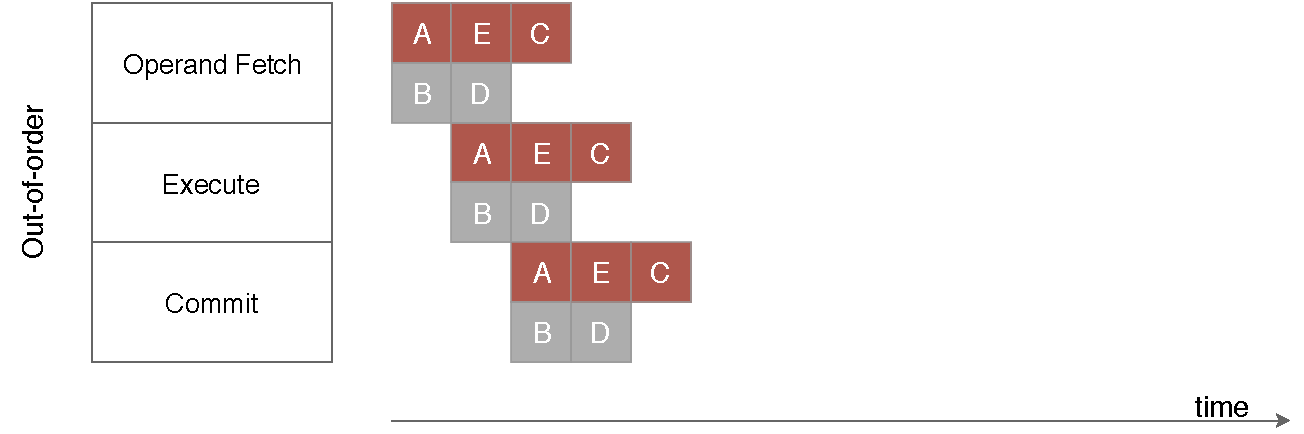
\includegraphics[width=\textwidth]{Source/SchedulingSchemes/Out-of-order.pdf}
	\caption{Out-of-order execution} 
	\label{fig-out-of-order}
\end{figure}
We can see in figure \ref{fig-superscalar} that, even with forwarding, the dependency between instructions C and B causes a bubble in the pipeline. In our simple model, where each instruction takes only one clock cycle, this may not seem like a major problem, but in reality, instruction can often take much longer. Load instructions that access memory are a good example of that. Cache misses can take over 100 cycles. If a following instruction needs that value, it has to wait for it. But there may be later instructions that do not depend on the load and could, in theory, be executed earlier. Out-of-order execution allows for this. \\
As long as we handle dependencies, we may execute an instruction earlier than the program order dictates, i.e. \textbf{out of order} to fill a gap in the pipeline, leading to an increase in IPC count. Figure \ref{fig-out-of-order} shows how, in our example, out-of-order execution can fill the gap in the pipeline between instructions B and C.\\


%\newgeometry{left=2cm,right=2cm,top=2cm,bottom=2cm}
%\restoregeometry


\newpage
\section{History and State of the Art}
As mentioned in the introduction, the primary paper that first described how multiple execution units could be used simultaneously was written by Robert Tomasulo in 1967 \cite{tomasulo}. The IBM System/360 Model 91 in 1966 used his algorithm for floating-point instructions but it took many years before superscalar execution was introduced to microprocessors.\\
The first one was probably the RS/6000 CPU, aka the POWER1, also developed by IBM in 1990 \cite{power1}. The time gap is at least partially due to the additional hardware that dynamic scheduling at runtime requires. In \cite{power1}, where Oeler and Blasgen from the IBM Research Division present the POWER1, they write:
\begin{quote}
	\textit{The realization of the system architecture in a full superscalar organization does require substantial hardware -- more than could fit on one chip in the available metal-oxide (CMOS) technology.}
\end{quote}
Technology was, however, just advanced enough at that point to fit the required hardware on \textit{six} chips, which is what the POWER1 did. It could issue up to four instructions in one cycle and started the very successful POWER series. \\
It is useful to study the POWER series in the context of this thesis, because it too implements a RISC ISA and because it spans almost three decades, from the first superscalar processors to today. At the time of writing, the POWER9 is even the basis for the fastest computer in the world, Summit \cite{top500}. \\
We can see in figure \ref{fig-POWER} that the number of instructions issued per clock cycle and the number of execution units has increased with almost every iteration. As transistors became smaller, hardware could get more complex. This allowed for wider pipelines.\\
The POWER processors saw the last decade of exponential clock rate increase until it started stagnating after around 2005 (see p.~\pageref{sec-physicallimits} for an essay on why this happened). This increased the pressure on computer architects to design pipelines with high throughput, as they could no longer rely on an increase in clock frequency to make up for it. \\
The table in figure \ref{fig-POWER} also shows two other trends, increased use of multithreading and multicore designs. These exploit thread-level parallelism, which is distinct from instruction-level parallelism and outside of the scope of this thesis.\\
\begin{figure} [htb!]
	\small  \sffamily
	\hfill \break
	\begin{tabularx} {\textwidth} {l C C C C C C C C C}
							& {\scriptsize \ttfamily POWER1}
							& {\scriptsize \ttfamily POWER2}
							& {\scriptsize \ttfamily POWER3}
							& {\scriptsize \ttfamily POWER4}
							& {\scriptsize \ttfamily POWER5}
							& {\scriptsize \ttfamily POWER6}
							& {\scriptsize \ttfamily POWER7}
							& {\scriptsize \ttfamily POWER8}
							& {\scriptsize \ttfamily POWER9} \\
		{\normalfont Release year} 		
							& 1990
							& 1993
							& 1998
							& 2001 
							& 2004
							& 2007
							& 2010
							& 2014
							& 2017\\
							&&&&&&&&&\\
		{\normalfont Clock rate (MHz)}	
							& 30 	%$\SI{30}{\MHz}$ 
							& 63 	%$\SI{63}{\MHz}$
							& 200 	%$\SI{200}{\MHz}$
							& 1300 	%$\SI{1.3}{\GHz}$
							& 2300	%$\SI{2.3}{\GHz}$
							& 4700  %$\SI{4.7}{\GHz}$
							& 5000  %$\SI{5.0}{\GHz}$
							& 5000  %$\SI{5.0}{\GHz}$
							& 4000  \\%$\SI{4.0}{\GHz}$\\
		{\normalfont \# Issues/cycle}
							& 4
							& 4 
							& 4
							& 5
							& 5
							& 7
							& 6
							& 10
							& 9\\
		{\normalfont \# Ex.~units/core}
						  	& 4
							& 6 
							& 7
							& 8
							& 8
							& 9
							& 12
							& 16
							& 28 \\
		{\normalfont \# Threads/core}
							& 1
							& 1 
							& 1
							& 1
							& 2
							& 2
							& 4
							& 8
							& 4/8\\
		{\normalfont \# Cores}
							& 1
							& 1
							& 1 
							& 2
							& 2
							& 2
							& 8
							& 12
							& 24/12\\
	\end{tabularx}
	\hfill \break
	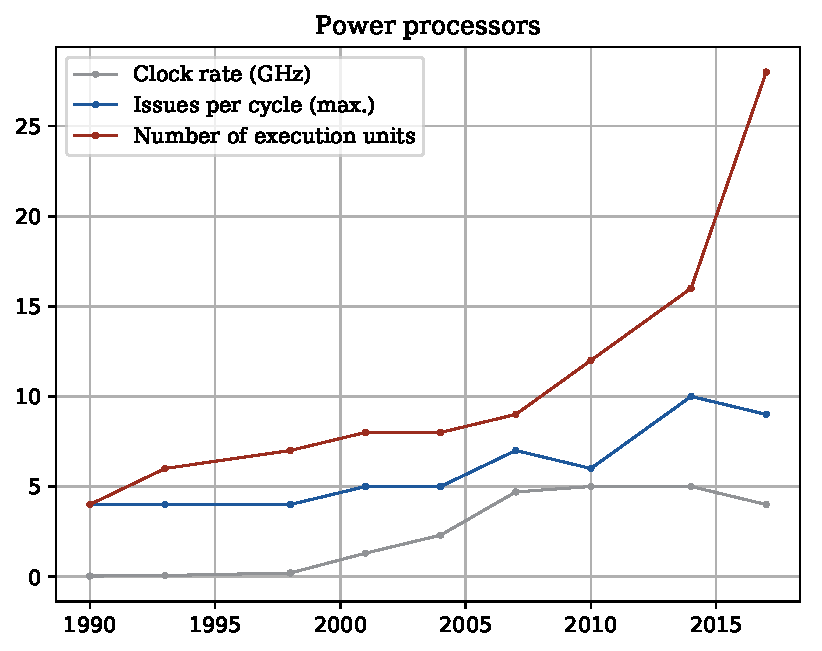
\includegraphics[width=\textwidth]{Source/POWER.pdf}
	
	\caption{\small The POWER series. Data from \cite{power1}, \cite{power2}, \cite{power3}, \cite{power4},
	\cite{power5}, \cite{power6}, \cite{power7}, \cite{power8} and
	\cite{power9}}%
	\label{fig-POWER}
\end{figure}%

To a small degree, superscalar processors already implement a simple form of out-of-order execution since they violate the original, sequential program order. But for a processor to be declared truly out-of-order, it needs to potentially be able to swap the program order of two instructions if the data flow permits it. The POWER1 was also probably the first microprocessor to support this \cite{power1}. It dispatches instructions in groups, inside of which execution can happen out-of-order. Later iterations loosened this group restraint. The POWER9 can track up to 256 operations out-of-order in every core (24 core version) \cite{power9}.\\
Eventually, all major processor developers introduced some form of superscalar out-of-order execution to their processors \cite{intelSM} \cite{amdSM}. It has become standard practice.\\

The next section will present a possible implementation of a simple superscalar out-of-order processor. It explains how new hardware structures make it possible for a processor to dynamically schedule instructions at runtime.



\begin{figure}[!p]
	\centering
	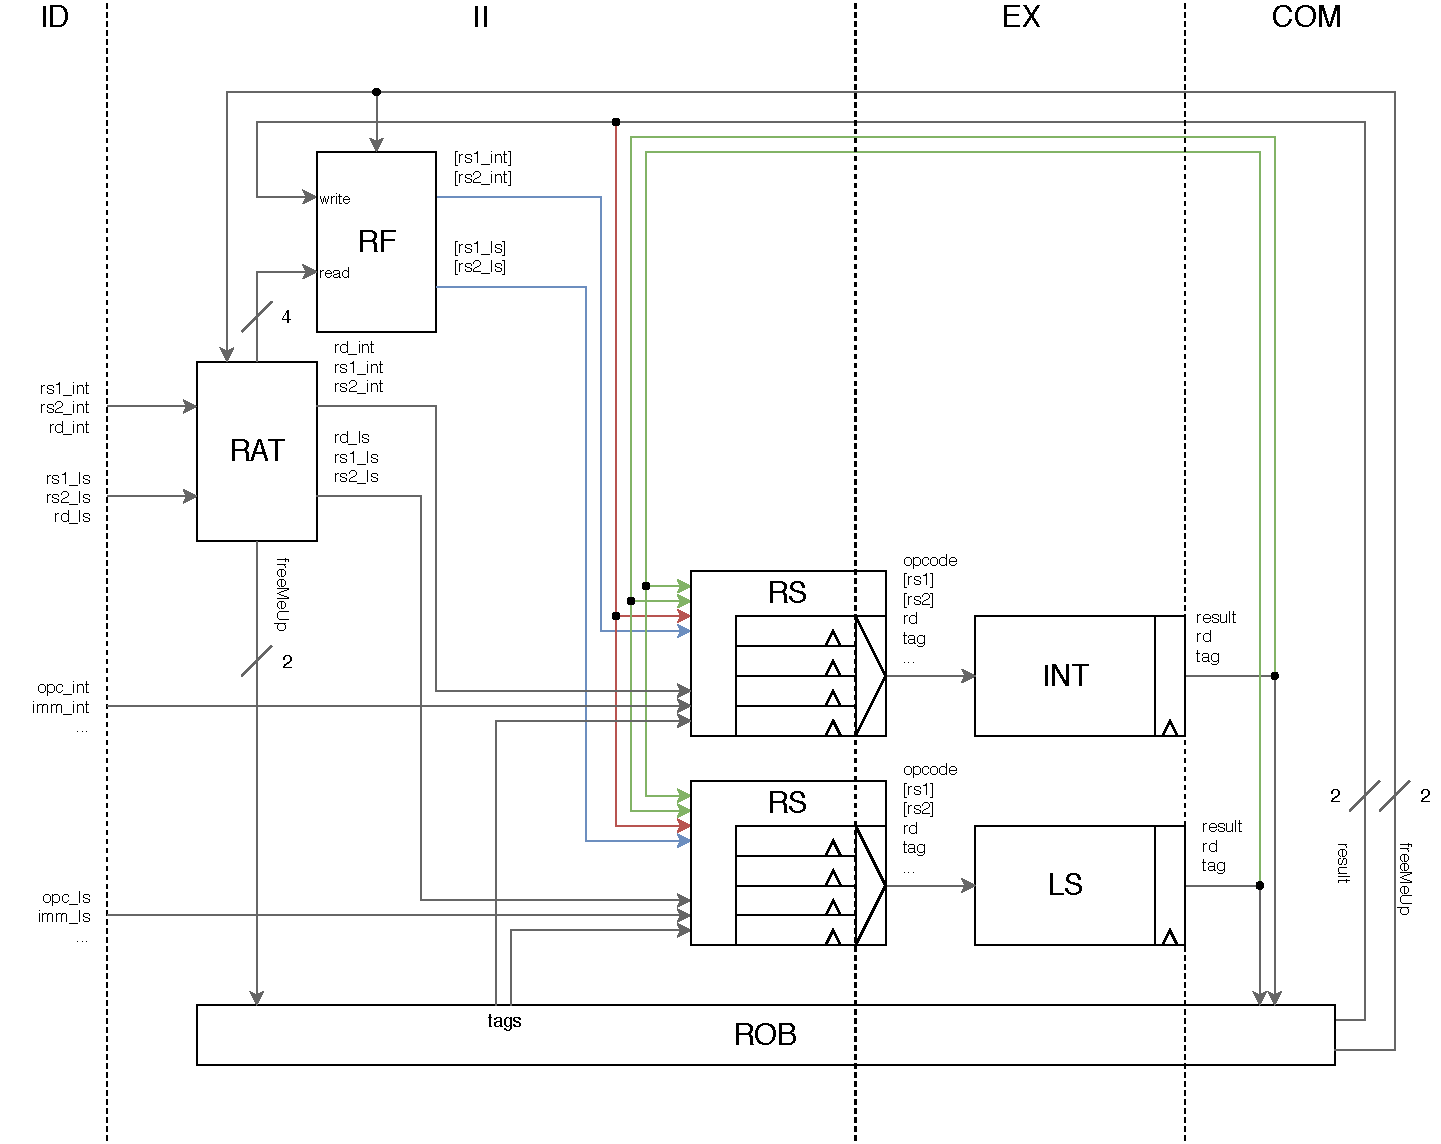
\includegraphics[height = \textwidth, angle = 90]{Source/pipeline.pdf}
	\caption{Pipeline design}
	\label{fig-pipeline}
\end{figure}
\newpage
\section{Design} \label{sec-design}
Figure \ref{fig-pipeline} shows a high-level diagram of the pipeline that I designed and implemented over the course of this thesis project.\\
To keep it simple, this pipeline only has one integer unit and one load-store unit (LS unit). The integer unit can only add two 64-bit values from registers and the LS unit can only load 64-bit values from memory. This is the functionality that is needed to run the LD and ADD instructions from the RISC-V ISA that I have introduced before. The integer unit takes one cycle for each ADD. The dummy LS unit also takes one cycle for a LD $90\%$ of the time. But in $10\%$ of cases, it takes ten cycles. This is supposed to simulate a cache miss. In those cases, the LS-unit blocks other LD instructions in the pipeline. LD instructions return random 64-bit values between $0$ and $1000$. \\

The general idea of the design is that instructions are sent to reservation stations (RS) where they wait until both of their source operands are available. Once they have them, they are executed, irrespective of their original program order. The results are buffered until they can be committed to the RF in-order. This is supposed to mimic an ideal dataflow engine, where there is no program order and instructions are executed as soon as they are ready to do so. \\

The first subsection will talk about this instruction flow step by step and then the second subsection will present the new modules in more detail.

\subsection{Pipeline stages and instruction flow}
Before I talk about pipeline stages, I should note that there are many different stage naming conventions. Some authors distinguish ``dispatch'' and ``issue'', others use them interchangeably. Similarly ``finish'', ``retire'' and ``commit'' often mean different things, but not always. I will use ``issue'' to refer to the stage in which instructions are moved from the ID stage to a reservation station. Instructions ``finish'' execution when their results are calculated. They are ``committed'' when their results are written to the register file.\\

\textbf{Instruction Decode (ID)}\\
The instruction decode stage is in charge of arranging instructions and their parts to make the next steps as easy as possible. It was not part of my thesis project to study this stage. I did, however, have to make certain assumptions about it to have well-defined input for the following stages.\\
My design demands that the ID stage delivers up to two instructions every cycle, but not more than one of each type (integer, load-store). Either, both or neither can be valid in any cycle. The design also currently requires the integer instruction to come before the load instruction in program order if both are valid in one cycle.\\

\textbf{Instruction Issue (II)}\\
Every clock cycle the instruction issue stage receives up to two instructions from the decode stage. The register alias table (RAT) is in charge of register renaming to eliminate false dependencies (see \ref{sec-RAT} for details). Once renamed, the register file (RF) attempts to read the source operands for both instructions. If they are available, their values are stored in the respective reservation station together with the rest of the instruction (destination register, opcode, immediate etc.). Reservation stations are simply bundles of registers where instructions wait for their source operands. Every execution unit has its own reservation station. The reorder buffer (ROB, see \ref{sec-ROB}) gives each instruction a tag, which is used to keep track of the program order of instructions.\\
Instructions that did not get both of their source operands from the RF wait in their reservation station until they have received both source operands from either the forwarding paths of the execution units or the commit path (see \ref{sec-RS} for details).\\

\textbf{Execute (EX)}\\
Whenever an execution unit is ready, it can start executing any one of the instructions in the reservation station that have all their source operands. \\
This now no longer has to happen in program order. It is possible for instructions to overtake other instructions in the reservation station if their source operands are available early enough. This prevents instructions from blocking independent instructions that are behind them in program order.\\

\textbf{Finish and Forward}\\
Once an instruction finishes execution, its result is written back to the reorder buffer using the tag it received in II (see \ref{sec-ROB}). The result is also forwarded to both reservation stations, in case it is the source operand of a waiting instruction.\\
This stage cannot be easily drawn in figure \ref{fig-pipeline} like the others. This is because its output register is a spot inside the ROB, which I decided to draw horizontally.\\

\newpage
\textbf{Commit (COM)}\\
In this step, results that have been written back to the ROB are committed in their original program order. This is possible because instructions were tagged before they were placed into reservation stations.\\

\textbf{Backwards flow control}\\
There are three reasons that can cause ID to be stopped:
\begin{enumerate}
	\item The ROB runs out of tags
	\item The reservation stations are full
	\item There are no more registers left for renaming (see \ref{sec-RAT})
\end{enumerate}
If any one of these happens, the ID stage needs to be stalled until enough instructions have been committed to free up space for new ones.

\subsection{New structures for superscalar out-of-order execution}
Even before they became superscalar, processors had register files and execution units. The RAT, the ROB and the reservation stations are the new, critical additions that make superscalar out-of-order execution possible. This subsection takes a closer look at how they work.

\subsubsection{The register alias table (RAT)} \label{sec-RAT}
\begin{wrapfigure} {H}{0.2\textwidth}
	\begin{minipage}{.2\textwidth}
		\begin{tabularx} {\textwidth} {R | X|}
			\cline{2-2}
			R1 		& P50	\\
			R2		& P2	\\
			R3		& P26	\\
			R4		& P4	\\
			R5		& P36	\\
			$\rightarrow$ R6		& P27	\\
			\cline{2-2} 
		\end{tabularx}
	\end{minipage}% 
	\caption{Possible RAT}
	\label{fig-possibleRAT}
\end{wrapfigure}
I introduced the general idea of register renaming in subsection \ref{sec-dependencies} but have not yet explained how it can be implemented. \\
There are 32 integer registers in the base RISC-V ISA, x0-x31, where x0 is hardwired to 0 \cite[p.~9]{riscv}. To implement register renaming effectively, the register file should have more physical registers than the ISA specifies. This version uses 64 physical registers so that they can be addressed with only one bit more. To clearly separate them, I will always use R0-R31 to refer to the architectural registers, and P0-P63 to refer to the physical registers. This is not a common naming convention but makes talking about register renaming much easier.\\

The essential unit that handles register renaming is the register alias table (RAT), which keeps track of the mapping between physical architectural registers. It also keeps a 64-bit list, that indicates which physical registers are currently being used and which ones are free. I will use the term RAT to refer both to the module that does the renaming and the actual mapping table it contains. The first few entries of that table may look like in figure \ref{fig-possibleRAT}. This would mean that R1 was mapped to P50, R2 to P2, R3 to P26 and so on. R0 will always be mapped to P0, which is always 0.\\
The architectural register number is used to index the table. It is therefore $\SI{32}{\bit}$ deep and $\log_2\SI{ 64}{bit} = \SI{6}{\bit}$ wide.\\

\textbf{Renaming registers}\\
Let us re-examine the example from earlier (see subsection \ref{sec-dependencies}):
\begin{assembly}
	\begin{tabularx} {\textwidth} {n o a a X}
		1 & LD  & R3 & 18(R1)	& \\
		2 & ADD & R5 & R3		& R2\\
		3 & LD  & R3 & 19(R1)	& \\
		4 & ADD & R6 & R3		& R2\\
	\end{tabularx}
\end{assembly}
We noted that there are true dependencies among the first two instructions and among the last two instructions. We also noted that even though instructions \texttt{3} and \texttt{4} are logically independent of instructions \texttt{1} and \texttt{2}, they still have to wait for them because of the reuse of R3.\\
We saw how this false dependency can be manually removed by renaming registers, but how can a CPU identify and resolve name dependencies \textit{at runtime}?\\

Before the code above is decoded, the RAT will at least contain information about R1 and R2 because they will be used in this code. They may simply be mapped to P1 and P2. In that case, the RAT would look like the table marked with 0 in figure \ref{fig-RAT}.
\begin{figure} [!htb] 
	\hspace{.1\textwidth}%
	\begin{minipage}{.2\textwidth}
		\begin{tabularx} {\textwidth} {R  C}
			& 0\\
		\end{tabularx}	
		\begin{tabularx} {\textwidth} {R | X|}
			\cline{2-2}
			R1 					  & P1\\
			$\rightarrow$ R2					  & P2\\
			R3					  & \\
			R4					  & \\
			R5					  & \\
			R6					  & \\
			\cline{2-2} 
		\end{tabularx}
	\end{minipage}% 
	\hspace{.1\textwidth}%
	\begin{minipage}{.2\textwidth}
		\begin{tabularx} {\textwidth} {R  C}
			& 1\\
		\end{tabularx}
	\begin{tabularx} {\textwidth} {R | X|}
		\cline{2-2}
		R1 					  & P1\\
		R2					  & P2\\
		$\rightarrow$ 
		R3					  & P3\\
		R4					  & \\
		R5					  & \\
		R6					  & \\
		\cline{2-2}
	\end{tabularx}
	\end{minipage}%
	\hspace{.1\textwidth}%
	\begin{minipage}{.2\textwidth}
		\begin{tabularx} {\textwidth} {R  C}
			& 2\\
		\end{tabularx}
	\begin{tabularx} {\textwidth} {R | X|}
		\cline{2-2}
		R1 					  & P1\\
		R2					  & P2\\
		R3					  & P3\\
		R4					  & \\
		$\rightarrow$
		R5					  & P4\\
		R6					  & \\
		\cline{2-2}
	\end{tabularx}
	\end{minipage}
	\\%
	\vspace{0pt}%
	\hspace{.1\textwidth}%
	\begin{minipage}{.2\textwidth}
		\begin{tabularx} {\textwidth} {R  C}
			& \\
			& 3\\
		\end{tabularx}
	\begin{tabularx} {\textwidth} {R | X|}
		\cline{2-2}
		R1 					  & P1\\
		R2					  & P2\\
		$\rightarrow$
		R3					  & P5\\
		R4					  & \\
		R5					  & P4\\
		R6					  & \\
		\cline{2-2}
	\end{tabularx}
	\end{minipage}%
	\hspace{.1\textwidth}%
	\begin{minipage}{.2\textwidth}
		\begin{tabularx} {\textwidth} {R  C}
			& \\
			& 4\\
		\end{tabularx}
	\begin{tabularx} {\textwidth} {R | X|}
		\cline{2-2}
		R1 					  & P1\\
		R2					  & P2\\
		R3					  & P5\\
		R4					  & \\
		R5					  & P4\\
		$\rightarrow$
		R6					  & P6\\
		\cline{2-2}
	\end{tabularx}
	\end{minipage}%
	\vspace{.5cm}
	\caption{RAT after each instruction}
	\label{fig-RAT}
\end{figure}
Now, after instruction \texttt{1} is decoded, the RAT will replace the source operand R1 with P1. It will also give R3 a new name. In this case, P3 is the next vacant register, so we can use that. The renamed instruction will now be:
\begin{assembly}
	\begin{tabularx} {\textwidth} {n o a a X}
		1' & LD & P3 & 18(P1)		& \\
	\end{tabularx}
\end{assembly}
So far this is not very interesting. We simply replaced R1, R2 and R3 with P1, P2 and P3. \\
For the ADD instruction, the RAT remaps the source registers as before. It also needs a new name for R5. The next free register is P4. Instruction \texttt{2} is renamed to:%
\begin{assembly}
	\begin{tabularx} {\textwidth} {n o a a X}
		2' & ADD & P4 & P3		& P2\\
	\end{tabularx}
\end{assembly}
The RAT now looks like the table marked with 2 in figure \ref{fig-RAT}.\\
Just like with the first LD, instruction \texttt{3} has its source register R1 renamed to P1. However, it also gets a new, unused destination register. In our case, P5 is the next free one. The RAT updates the mapping for R3 (see figure \ref{fig-RAT}) and the renamed instruction is:
\begin{assembly}
	\begin{tabularx} {\textwidth} {n o a a X}
		3' & LD & P5 & 19(P1)		& \\
	\end{tabularx}
\end{assembly}
Instruction \texttt{4} now uses the \textit{new} name for R3, which is P5 instead of P3. Its destination is renamed to P6, the next free physical register:
\begin{assembly}
	\begin{tabularx} {\textwidth} {n o a a X}
		4' & ADD & P6 & P5		& P2\\
	\end{tabularx}
\end{assembly}
We can now observe that the renamed instructions \texttt{1'-4'} have no false dependencies, just like the manually renamed example in \ref{sec-dependencies}.\\
To summarize, the procedure for renaming registers of an instruction is:
\begin{enumerate}
	\item Replace architectural source registers with the mapped physical registers using the RAT
	\item Replace the architectural destination register with a new, vacant physical register. Update the RAT\\
\end{enumerate}

\newpage
\textbf{Freeing registers again}\\
If we always pick a new, free destination physical register for each instruction, we will eventually run out of registers. We need a mechanism that frees registers again at some point. But when can a register be safely used again?\\
Let us revisit the code from before:
\begin{assembly}
	\begin{tabularx} {\textwidth} {n o a a X}
		1 & LD  & R3 & 18(R1)	& \\
		2 & ADD & R5 & R3		& R2\\
		3 & LD  & R3 & 19(R1)	& \\
		4 & ADD & R6 & R3		& R2
	\end{tabularx}%
\end{assembly}%
which after renaming became:
\begin{assembly}
	\begin{tabularx} {\textwidth} {n o a a X}
		1' & LD & P3 & 18(P1)	& \\
		2' & ADD & P4 & P3		& P2\\
		3' & LD & P5 & 19(P1)	& \\
		4' & ADD & P6 & P5		& P2
	\end{tabularx}%
\end{assembly}%
In the original code, instruction \texttt{3} overwrites R3. Later instructions will not have access to, and therefore will not depend on the old value of R3. Through renaming, the ``old'' value is saved in P3 and the ``new'' value in P5. This means that once all instructions up to instruction \texttt{3} are executed, the value in P3 will definitely never be needed again. Since we commit instructions in program order, we can safely free P3 once instruction \texttt{3} is committed. To do this, I use a so-called \textbf{free-me-up tag}. In figure \ref{fig-RAT} we can see that before instruction \texttt{3} is renamed, the RAT can check which physical register was mapped to R3 before, in this case, P3. The RAT then sets the free-me-up tag of instruction \texttt{3} to P3, before it remaps R3 to P5. Once instruction \texttt{3} is about to commit, the free-me-up tag is sent back to the RAT, so that it can update the free list.\\

In figure \ref{fig-pipeline} we can see that the free-me-up tag is also sent back to the RF. This is because the RF keeps information on whether the value in a register is valid yet. Once we free up a register to reuse it, whatever was in this register before becomes invalid. So the RF needs to know when we repurpose a physical register.\\

We can think of setting the free-me-up tag as step 3 of register renaming:
\begin{enumerate}
	\item[3.] If the architectural destination register was mapped to another physical register before, set the old one as the free-me-up tag
\end{enumerate}


\newpage 
\subsubsection{The reorder buffer (ROB)} \label{sec-ROB}
The reorder buffer (ROB) tags instructions in program order so that they can be \textbf{committed in order} even when their actual execution order is completely different. After instructions are executed, their results are written back to the ROB, where they wait to be committed. So the ROB has three major functions:
\begin{enumerate}
	\item Tag instructions in-order when they are placed in reservation stations
	\item Save instruction results (possibly out-of-order) until they can be committed
	\item Commit results in-order
\end{enumerate}
These three functions need to happen simultaneously in every clock cycle. Because of how the ROB is connected to every pipeline stage, I decided to draw it as running in parallel to all the other modules in figure \ref{fig-pipeline}. In other depictions, it is often drawn as a buffer between the execution units and the register file.
\begin{figure}[H]
	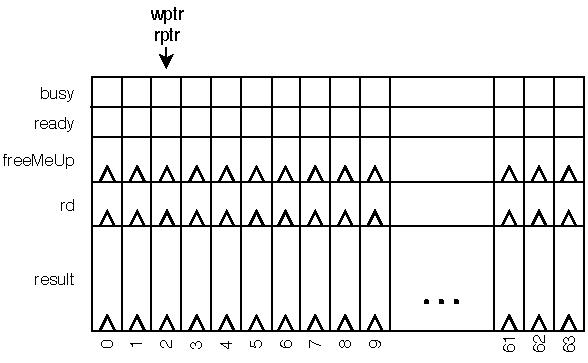
\includegraphics[width=\textwidth]{Source/ROB/ROB-Empty.pdf}
	\caption{Empty ROB}% 
	\label{empty}
\end{figure}%
The ROB can be thought of as an array of registers for instruction results and their destination registers (rd). It also saves the free-me-up tag of each instruction (see \ref{sec-RAT}). We can draw this structure as in figure \ref{empty}. The write pointer (wptr) always points to the next free spot in the ROB and doubles as the tag that is given to incoming instructions when they are issued (in-order) to a reservation station. That location in the ROB is then marked as busy. The read pointer (rptr) always points to the oldest instruction. This is the head of the commit queue. Figure \ref{partiallyBusy} shows a ROB with six busy slots before any of those instructions finished execution. The free-me-up tag and the destination register are known at this point. 
\begin{figure}[H]
	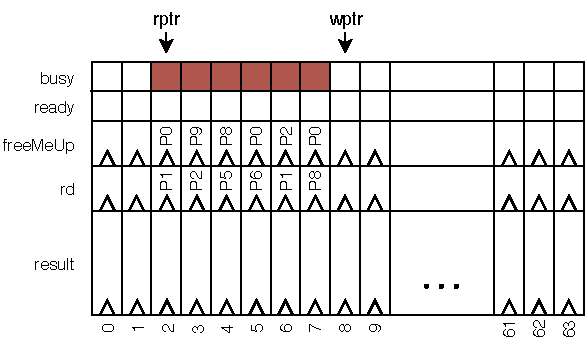
\includegraphics[width=\textwidth]{Source/ROB/ROB-Busy.pdf}
	\caption{Partially busy ROB}%
	\label{partiallyBusy} 
\end{figure}%
\begin{figure}[H]
	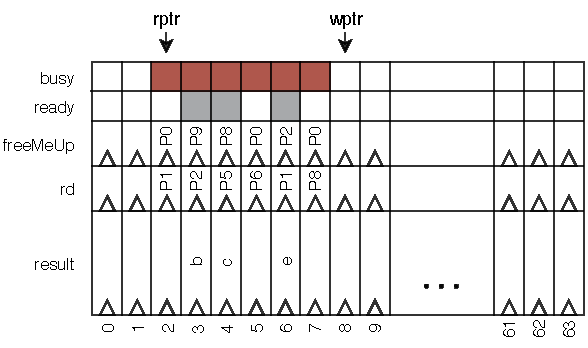
\includegraphics[width=\textwidth]{Source/ROB/ROB-PartiallyReady.pdf}
	\caption{ROB with some entries that are ready to commit} 
	\label{partiallyReady}
\end{figure}%
When an instruction has finished execution, its result is written to the ROB by matching the tag that the instruction got in II. Reservation stations allow for instructions to be executed out-of-order, so the ROB needs to be able to write any result register in each cycle. Figure \ref{partiallyReady} illustrates one possible situation, where three of the six instructions have finished execution and written their results to the ROB.
\begin{figure}[H]
	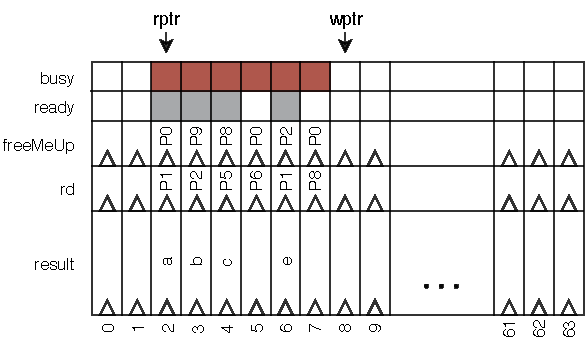
\includegraphics[width=\textwidth]{Source/ROB/ROB-Ready.pdf}
	\caption{ROB that is about to commit} 
	\label{aboutToCommit}
\end{figure}%
\begin{figure}[H]
	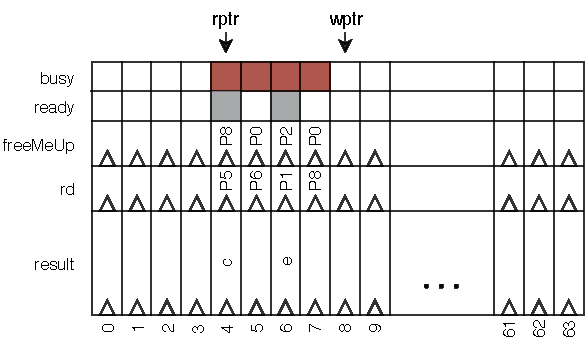
\includegraphics[width=\textwidth]{Source/ROB/ROB-AfterCommit.pdf}
	\caption{ROB after commit} 
	\label{afterCommit}
\end{figure}%
In this case, no results can be committed yet because the instruction at rptr is not ready to commit yet. Once the two instructions at rptr and rptr+1 are ready to commit, like in figure \ref{aboutToCommit}, their results are written to the register file. The rptr advances two spots and the two locations are marked as not busy and not ready. In our example, the resulting ROB may look like in figure \ref{afterCommit}.\\
In practice, the ROB will tag new instructions, collect results and commit ready instructions every clock cycle, rather than in sequence like in this example. \\

\textbf{Other tags and values in the ROBs}\\
One can easily see that the busy tag is not actually necessary. It is directly determined by the location of wptr and rptr. However, it can make the ROB easier to understand and debug. Similarly, my SystemVerilog implementation also saves the opcode of each instruction. This makes waveforms, in particular, much easier to read (see section \ref{sec-results}) and these redundant values can easily be removed in later stages of development.\\ 

\subsubsection{The reservation stations} \label{sec-RS}
In this design, both reservation stations can keep up to four instructions. Each slot contains space for the following information:
\begin{itemize}
	\item The register address of the source operands rs1 and rs2 
	\item The value of the source operands rs1 and rs2
	\item A valid tag for each source operand that indicates if it has been received yet
	\item Other instruction parts that come directly from ID (opcode, immediate, etc.)
	\item The tag from the ROB
	\item A free tag that indicates if the slot is being used
\end{itemize}
An instruction is ready for execution once it has both source operands, that is when both valid tags are set. There are three ways an instruction can receive its source operands:
\begin{enumerate}
	\item From the RF:\\
	If a source operand has already been written back to the RF by the time an instruction is issued to a reservation station, the value is copied into the reservation station in the same cycle as the instruction. This is the blue path in figure \ref{fig-pipeline}.
	\item From the forwarding paths:\\
	The reservation stations listen in on the results paths from execution units to the ROB. Every clock cycle, the destination register of a new result is checked against all the source registers of the waiting instructions. These are the green paths in figure \ref{fig-pipeline}.
	\item From the commit path:\\
	The reservation stations also check against destination registers of instructions that are being written back to the RF. This has to happen both for waiting instructions and for instructions just being issued. In figure \ref{fig-pipeline}, this is the red path. 
\end{enumerate}
The four slots are numbered and new instructions are placed into the first free one. If several instructions are ready for execution, the first ready one is chosen for execution. 

\newpage
\begin{center}
	This page has been intentionally left blank 
\end{center}

\newpage
\section{Results} \label{sec-results}
The design presented in section \ref{sec-design} was implemented in around $1300$ lines of IEEE 1800-2009 SystemVerilog code. This includes several test cases implemented as tasks that can be called in the top module. The code was developed and tested using the Incisive Enterprise Simulator from Cadence Design Systems. \\

During the course of this thesis, I also wrote a python script that takes SystemVerilog code for a module and creates the skeleton code for a corresponding test bench. It instantiates the module, a clock and all the regs and wires that are necessary to connect the test bench to the module. It can be found at \url{github.com/amanda-matthes/Testbench-Generator-for-SystemVerilog-Modules} and may be useful for further development.\\

To expedite testing, I also created several .tcl.svcf command scripts for SimVision. These can be sourced to automatically arrange and colour waveforms in useful ways. They also include definitions of mnemonics. Mnemonics translate the original binary waveforms into text, where appropriate. This means that instead of the 7-bit opcode $0110011$, the waveform will read ``ADD'' and instead of the architectural register address $10110$, the waveform will read ``R22'', etc. Used mnemonics include:
\begin{itemize}
	\item R0-R31 instead of 00000-11111 for architectural registers
	\item P0-P63 instead of 000000-111111 for physical registers
	\item ADD and LD instead of the opcodes 0110011 and 0000011 \cite[p.~104f]{riscv}
	\item BUSY, FREE, VALID, RESET, FULL and STOP instead of 0 and 1, where appropriate\\
\end{itemize}

In this section, I will demonstrate the core functions of my design by looking at how the simulation handles certain inputs. To do this, this section includes waveforms from SimVision of selected signals for each example. They make use of the above-mentioned mnemonics.

\newpage
\subsection{Superscalar execution}
I first want to show that my design can, in fact, achieve superscalar execution, with $\text{IPC} = 2$. To do this, I fed the pipeline one ADD and one LD instruction at the same time. \\

Figure \ref{fig-superscalarity} shows selected waveforms that demonstrate how both instructions pass the pipeline stages at the same time. \\
The first signal is the clock, which I set to a period of $\SI{20}{\ns}$. The next four signals are the inputs. For this demonstration, the exact instructions are uninteresting. It is, however, necessary that they are of different types so that they can be executed in parallel by different execution units. I coloured the LD signals blue to distinguish them from the ADD signals in red. To ensure that the input was valid at the positive clock edge, I always manipulated it at the negative clock edge.\\
The next four signals show the first entry of the reservation station of the integer and the load-store unit, respectively (INT RS and LS RS). At the next positive clock edge ($\SI{70}{\ns}$), we can see that these are loaded with the instructions. I ensured that all source operands were available in the RF so that both instructions could load them in the same cycle and start execution in the next. \\
At the next positive clock edge ($\SI{90}{\ns}$), the reservation stations are freed again and the functional units start execution. Because this is a simulation at the register-transfer level (RTL), we do not see an execution delay and the output is valid immediately. In this case, there was a cache hit which means that the result of the load was available in the next clock cycle.\\
We can see that the ROB saved the instructions at the same time as the reservation stations ($\SI{70}{\ns}$). Once they finish execution ($\SI{110}{\ns}$), their results are written to the ROB. This also flags those ROB entries as ``ready to commit''. In the next clock cycle (starting at $\SI{130}{\ns}$) those results are written back to the RF. The ROB entries are freed again and one cycle later, the results are available in the RF. \\

This shows that, in theory, this design can execute two instructions every clock cycle if we can schedule one ADD and one LD in every cycle and there are no cache misses.

\begin{figure}[!p]
	\centering
	\includegraphics[width=\textwidth, trim = {1.5cm 1.5cm 1.5cm 1.5cm}]{Source/Waveforms/superscalarity.eps}
	\caption{Superscalar execution} 
	\label{fig-superscalarity}
\end{figure}

\newpage

\subsection{Register renaming}
I now want to demonstrate register renaming. In section \ref{sec-RAT}, I showed how this code:
\begin{assembly}
	\begin{tabularx} {\textwidth} {n o a a X}
		1 & LD  & R3 & 18(R1)	& \\
		2 & ADD & R5 & R3		& R2\\
		3 & LD  & R3 & 19(R1)	& \\
		4 & ADD & R6 & R3		& R2
	\end{tabularx}%
\end{assembly}%
can be renamed to this code:
\begin{assembly}
	\begin{tabularx} {\textwidth} {n o a a X}
		1' & LD & P3 & 18(P1)	& \\
		2' & ADD & P4 & P3		& P2\\
		3' & LD & P5 & 19(P1)	& \\
		4' & ADD & P6 & P5		& P2
	\end{tabularx}%
\end{assembly}%
to resolve false dependencies using two simple rules. I want to demonstrate that this is in fact what the design does.\\
To execute the code above, we first need to load the registers R1 and R2. I did this with:
\begin{assembly}
	\begin{tabularx} {\textwidth} {n o a a X}
		& LD & R1 & 0(R0) &\\
		& LD & R2 & 0(R0) &\\
	\end{tabularx}
\end{assembly}
The source register and the immediate are not important since loads return random values anyway, so I set them to zero.\\ 
As before, I always changed signals at the negative clock edge to ensure that they were stable at the next positive one. I always applied only one instruction every clock cycle, so that we could see the RAT after each instruction renaming. The result is shown in figure \ref{fig-renaming}.\\
The red waveforms show the integer input which consists of the important instruction parts and the corresponding valid signal. Our code has two integer instructions. Instruction \texttt{2} is issued at $\SI{130}{\ns}$ and instruction \texttt{4} at $\SI{170}{\ns}$. The first one is quite easy to read in the waveforms, but the second one seems to be missing some parts. This is simply because the opcode and both source registers have stayed the same and the waveform viewer only lets us see change. \\
Similarly, the blue waveforms show the load-store input. First, R1 and R2 are loaded, then R3 and, after the first ADD, R3 again, but this time with a different immediate.\\
The last six lines show the first few entries of the RAT. We can compare this with figure \ref{fig-RAT} and find that the simulation behaves exactly as predicted. 

\begin{figure}[!p]
	\centering
	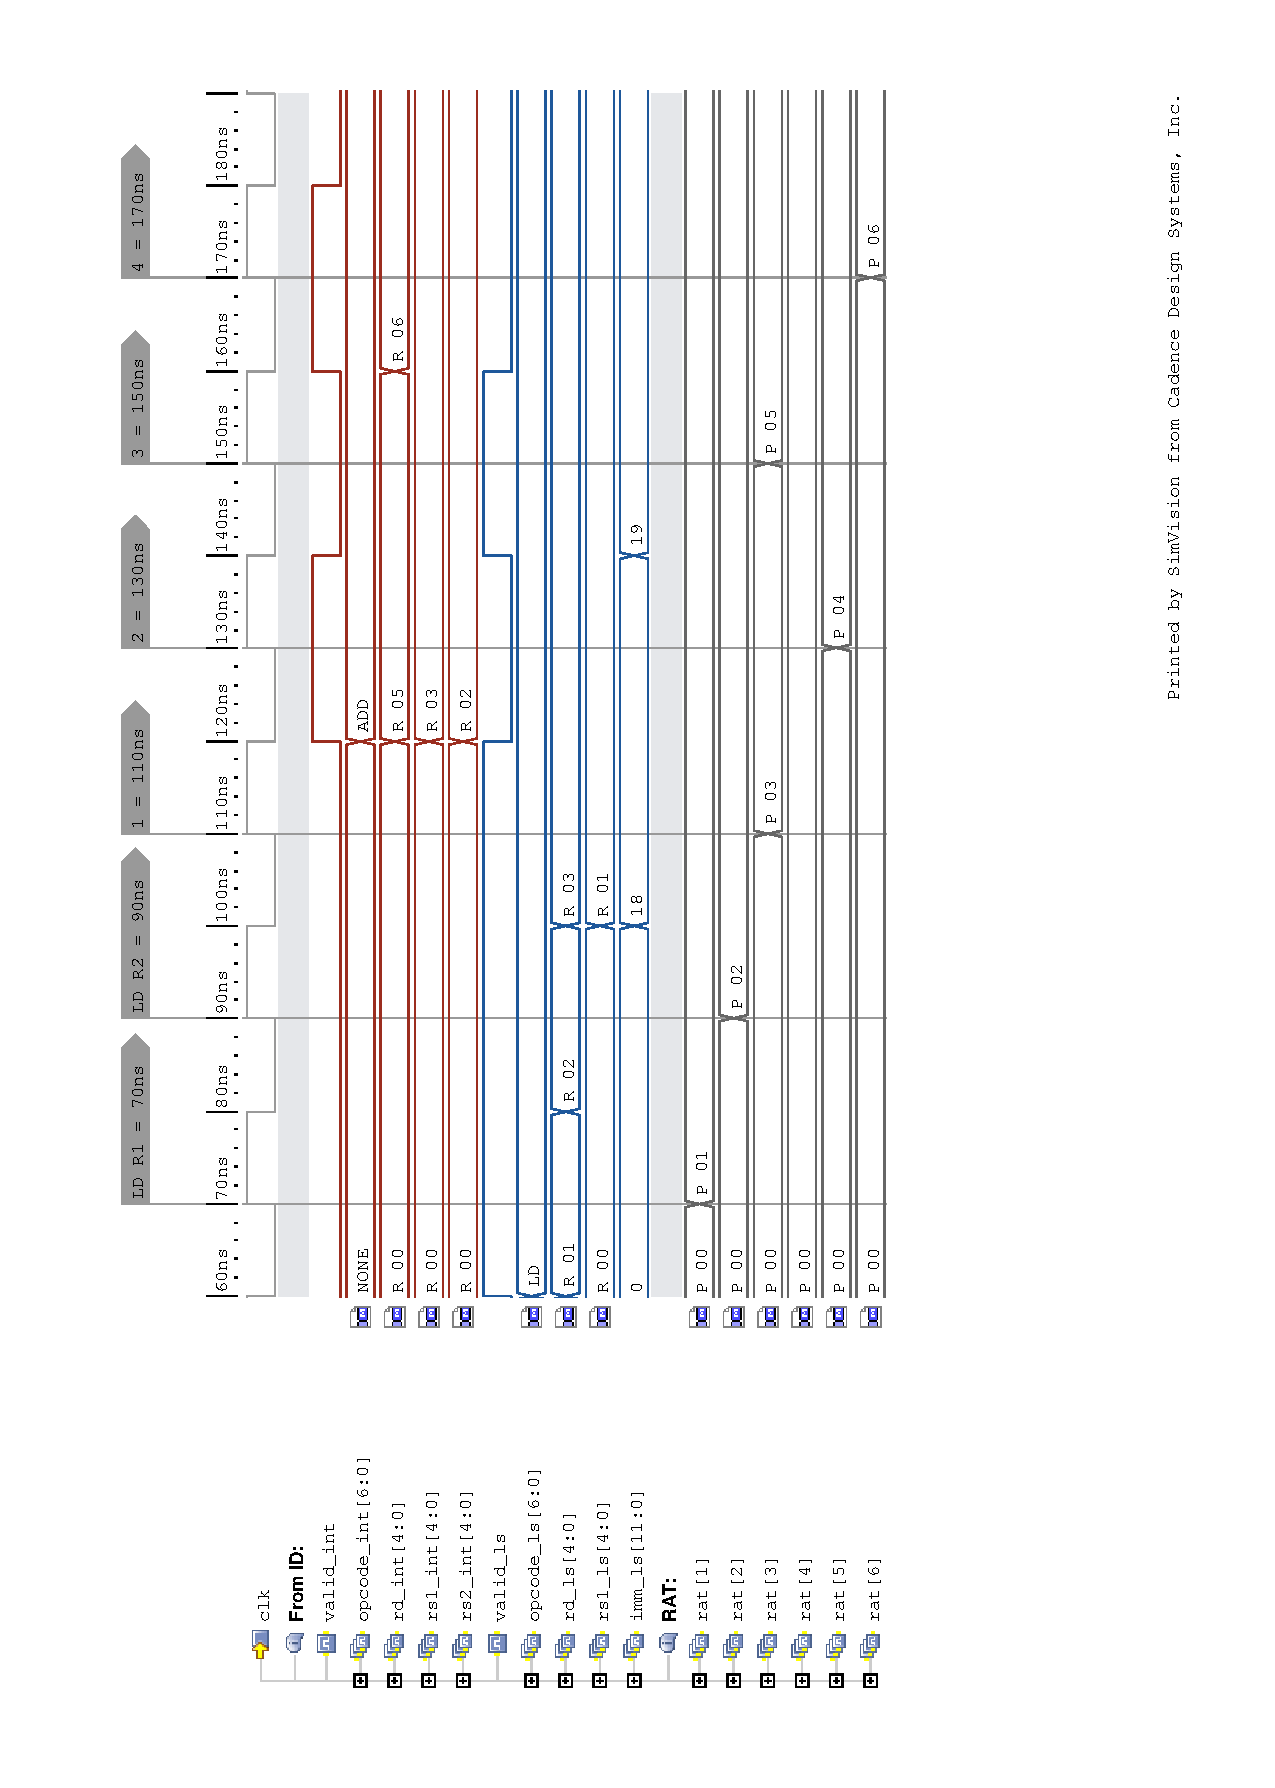
\includegraphics[width=\textwidth, trim = {1.5cm 1.5cm 1.5cm 1.5cm}]{Source/Waveforms/renaming.eps}
	\caption{Register renaming} 
	\label{fig-renaming}
\end{figure}

\subsection{Waiting for source operands and forwarding}
I now want to show how an instruction waits in its reservation station until it receives both its source operands. To do this, I executed the following instructions:
\begin{assembly}
	\begin{tabularx} {\textwidth} {n o a a X}
		1 & LD  & R1 & 0(R0)	& \\
		2 & LD  & R2 & 0(R0)	& \\
		3 & ADD & R3 & R1		& R2\\
	\end{tabularx}%
\end{assembly}%
This code loads R1 and R2 with random values and then adds them together. Figure \ref{fig-waiting} shows the result. \\
The first few signals simply show the input from the ID stage. As before, I use red for signals associated with integer operations and blue for load-store signals. The next section of waveforms shows what the LS unit outputs. We can see that the first LD returns the value 73 in the clock cycle starting at $\SI{90}{\ns}$, before the ADD instruction is even issued. This result is written back to the ROB at $\SI{110}{\ns}$ and then at $\SI{130}{\ns}$ is committed to the RF. These are the next three signals. \\
The last few signals show what happens inside the integer reservation station. While the first load is writing its result to the ROB, the ADD instruction is sent to the reservation station. In this case, R1 and R2 were simply renamed to P1 and P2 (see \ref{sec-RAT}). The register file had not been written yet and so neither rs1 nor rs2 is valid at this point. But when the result of the first LD is committed, it is also forwarded back to the reservation station (red path in figure \ref{fig-pipeline}). The 73 is copied into the reservation station (rs1\_content) and the valid tag is set (rs1\_valid).\\
The second LD is issued one cycle after the first which means that it starts execution when the first LD finishes it, at $\SI{110}{\ns}$. But this time there was a cache miss. Recall that I declared those to take ten cycles, that is $10 \times \SI{20}{\ns} = \SI{200}{\ns}$. At $\SI{310}{\ns}$ the LS unit returns the value 428, which this time can be directly forwarded to the reservation station (green path in figure \ref{fig-pipeline}). This means that the ADD instruction can start execution at $\SI{330}{\ns}$, before the value of P2 has even been committed.\\

The next subsection demonstrates how placing instructions into reservation stations like this enables out-of-order execution.


\begin{figure}[!p]
	\centering
	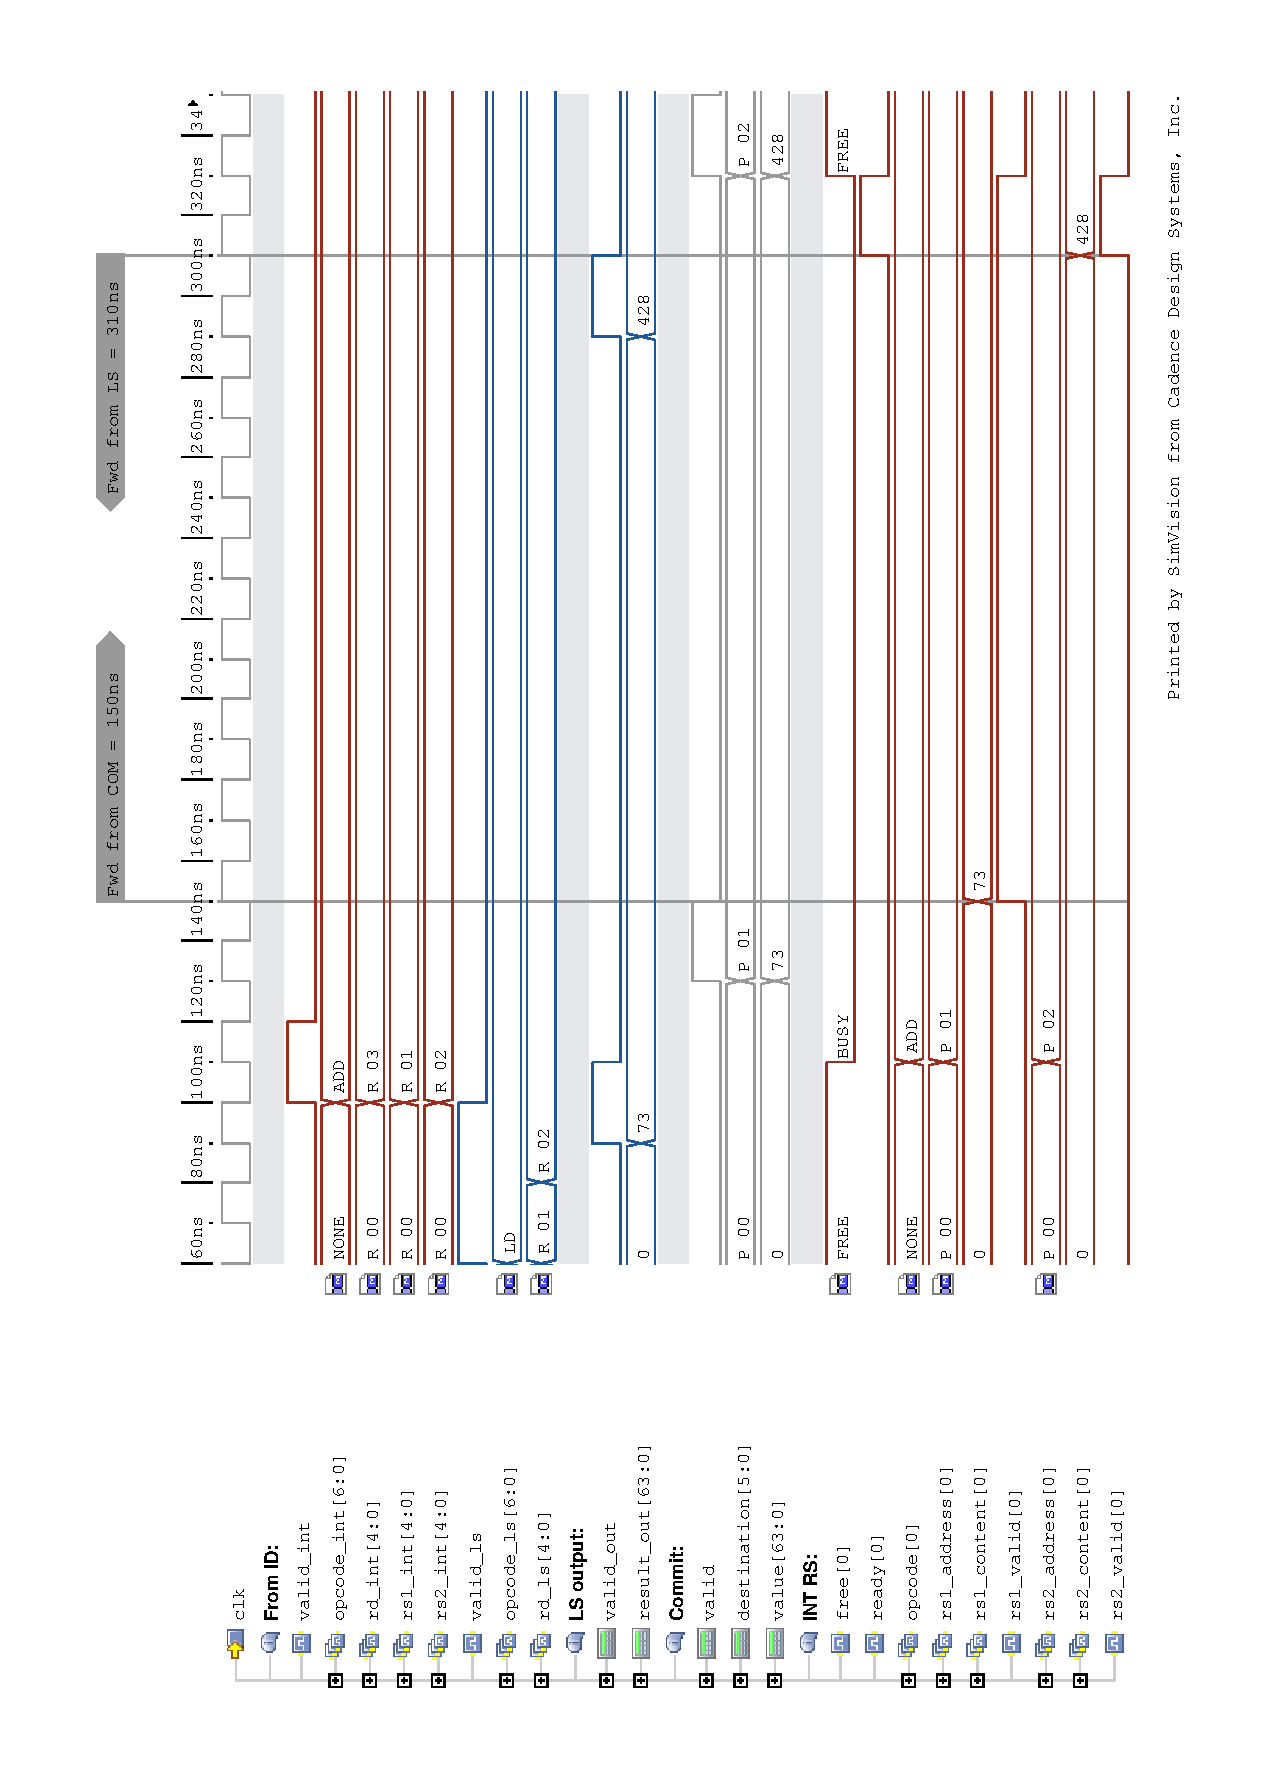
\includegraphics[width=\textwidth, trim = {1.5cm 1.5cm 1.5cm 1.5cm}]{Source/Waveforms/waitingForSourceOps.eps}
	\caption{Waiting for source operands in reservation stations} 
	\label{fig-waiting}
\end{figure}

\newpage
\subsection{Out-of-order execution}
Building on the example from the last subsection, I now want to show how an instruction can overtake a stalling instruction in front of it. \\
Let us revisit the code from before:
\begin{assembly}
	\begin{tabularx} {\textwidth} {n o a a X}
		1 & LD  & R1 & 0(R0)	& \\
		2 & LD  & R2 & 0(R0)	& \\
		3 & ADD & R3 & R1		& R2\\
	\end{tabularx}%
\end{assembly}%
We have seen how the ADD instruction waits in the first slot of the integer reservation station for both of its source operands. \\
I am now introducing a second ADD instruction, two cycles after the first:
\begin{assembly}
	\begin{tabularx} {\textwidth} {n o a a X}
		  & ADD & R4 & R1		& R1\\
	\end{tabularx}%
\end{assembly}%
This one only needs the result of the first LD to execute. \\
Figure \ref{fig-ooo} shows the first two slots of the integer reservation station. I set up the simulation so that the two LD instructions would behave as before. That is, return the same values and have one cache hit and one cache miss. This time, I used the colours red and blue to distinguish signals associated with the two source operands. \\
We can see that the second ADD is loaded into the reservation station just as the first LD commits its result ($73$) at $\SI{150}{\ns}$. The value is forwarded to both ADD instructions. As before, the second LD causes a cache miss and so rs2 of the first ADD takes another 10 cycles to become available. The second ADD instruction, however, only needs the first result. It can start execution at $\SI{170}{\ns}$, many cycles before the first ADD, even though it is behind it in program order. This is out-of-order execution. \\
The second ADD still needs to wait in the ROB for the first one to finish before it can commit in-order to the RF. But its result can be forwarded to waiting instructions many cycles before that. Furthermore, we could imagine up to nine more ADD instructions to execute while the first one still waits for its source operand. This is how out-of-order execution can speed up computers.


\begin{figure}[!p]
	\centering
	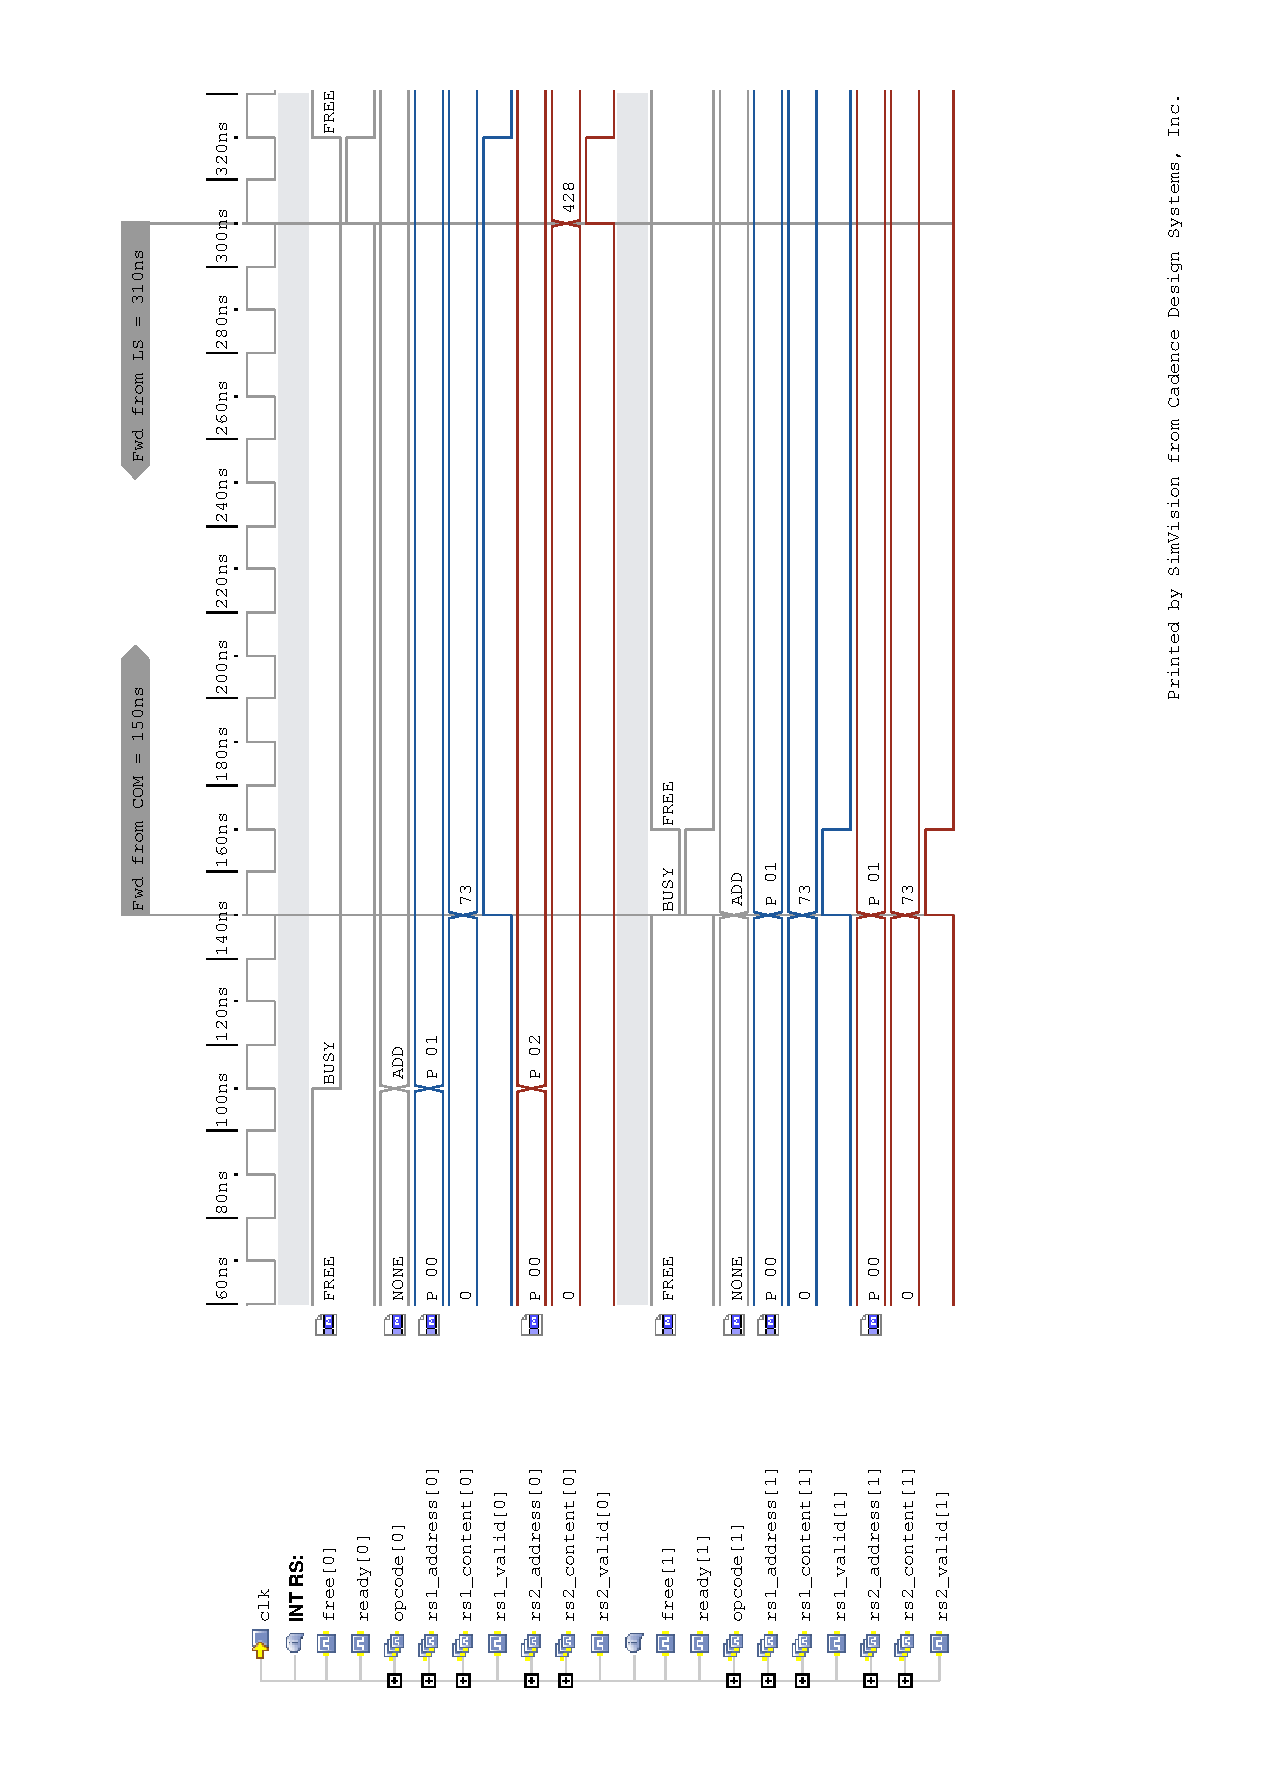
\includegraphics[width=\textwidth, trim = {1.5cm 1.5cm 1.5cm 1.5cm}]{Source/Waveforms/outOfOrder.eps}
	\caption{Instruction overtaking stalling instruction inside reservation station} 
	\label{fig-ooo}
\end{figure}


\newpage
\section{The limits of superscalar execution} \label{sec-superscalarLimits}
My design is a very simple prototype that can at most issue/commit two instructions per clock cycle. But we can easily imagine how this design could be scaled up to many more execution units, each with their own reservation station. There are two main reasons for why this is only useful to a certain degree. \\
The first point is that every piece of code inherently only has a few instructions that can be executed at any point. This is the data-flow limit. Since 1970, researches have made many different educated guesses on the limit of ILP in code, ranging from 2 to 50 \cite[p.~24]{lipastiShen}. This value is heavily application dependent and was generally underestimated before the introduction of speculative execution using branch prediction. A basic block is a piece of code with no branches. Without branch prediction, ILP could only be exploited inside these small basic blocks. Better branch prediction means that the amount of code across which ILP can be used increases. But even with advanced branch predictors, there will always be a hard limit (see section \ref{sec-outlook} for how data value speculation could help). \\
The second problem is that at some point, the hardware will become so complex that the potential speed-up is negated. Critical points include:
\begin{itemize}
	\item \textbf{The IF stage}\\
		The number of instructions that can be fetched in a cycle is limited by the size and architecture of the instruction cache and its cache lines. Misalignment and control dependencies also limit this stage. 
	\item \textbf{The RF}\\
		A broad pipeline requires a heavily multi-ported RF. This greatly affects area and power consumption \cite[p.~4]{surveyOfRF}.
	\item \textbf{The forwarding logic}\\
		The complexity of the forwarding paths grows both with the number of execution units and the number of slots in the reservation stations.
	\item \textbf{The ROB}\\
		A broader pipeline means that the ROB needs to be able to tag and commit more instructions. The bigger problem is that it also needs to potentially save more results every clock cycle. This is a random access (see section \ref{sec-ROB}) and faces the same restrictions as the RF. 
\end{itemize}
Because of these issues, manufacturers in the mid-noughties started focusing on thread-level parallelism \cite[p.~245f]{Hennessy}. But figure \ref{fig-POWER} shows that exploiting ILP has continued to be important, even as the number of cores and threads increased.


\newpage
\section{The dangers of out-of-order speculative execution: Meltdown and Spectre} \label{sec-oooDangers}
The separation of the architectural state and the micro-architectural (physical) state of a machine has opened up new security risks. Most notably, 2018 saw the disclosure of \textbf{Meltdown} and \textbf{Spectre}. These vulnerabilities allow attackers to access all memory in a system.\\

If an instruction accesses memory that it is not allowed to read, an exception is raised. However, the exception is only raised when the instruction is committed. Until then, the value can be used by \textbf{transient instructions}. These are instructions that will not be committed because of the exception. They cannot affect the correctness of the program and therefore used to be regarded as harmless. However, while these transient instructions cannot affect the architectural state of the machine, i.e. the register file, they \textit{can} affect the micro-architectural state of for example the cache. An attacker can use the illegally accessed value to calculate a memory address and load that cache-line into the cache. By timing the access time to that cache-line, the attacker can reconstruct the address and thereby the secret value. This is Meltdown. \cite{meltdown}\\

Spectre makes use of \textbf{speculative execution}. If there is a conditional branch in the instruction flow, modern processors will speculatively execute following instructions until the condition is evaluated. If the branch direction was mispredicted, the instructions are discarded. If not, the processor just saved time. Out-of-order execution can make speculative execution more prominent because the outcome of a conditional branch instruction may depend on preceding instructions that have not been completed yet. The branch predictor can be trained to predict a certain outcome. If a branch is taken 100 times in a row, it will likely be taken again. An attacker can exploit this by hiding instructions that use secret information behind a branch that is not taken. The branch predictor can be trained to mispredict this branch and the processor will be tricked to execute these instructions. Similarly to Meltdown, there now is a time window in which the micro-architectural state can be used to leak secret information. \cite{spectre}\\

The underlying reason for these vulnerabilities is the discrepancy between the architectural and the physical state of modern processors. Computer architects now need to carefully consider the visibility of the micro-architectural state.

\newpage
\section{Conclusion and Outlook} \label{sec-outlook} \label{sec-conclusion}

I have presented one possible implementation of a simple, superscalar out-of-order processor. I demonstrated the major advantages and challenges that these techniques bring. 

\subsection{Further work}
The aim of this thesis was to design hardware structures to allow for superscalar out-of-order execution. I did not attempt to build a complete RISC-V processor. There is still work left to do to achieve a fully functioning CPU. This subsection lists some of this necessary work as well as other improvements that can be made to this design. \\

\textbf{Support for other instructions}\\
	The processor is currently only able to support ADD and LD instructions from the RISC-V instruction set. Adding support for the rest will change the output registers of the ID stage. The processor will also need to handle the immediate value which replaces one of the source operands. This version simply drags it along, since it does not affect the output. Support for floating-point instructions will require a second RF and more renaming logic.\\

\textbf{Speculative execution}\\
	My design assumes a linear instruction flow without branches and control dependencies that stem from them. Branch prediction with speculative execution has become the norm in processors and provides a significant speed-up. It will eventually need to be incorporated.\\
	
\textbf{Exceptions}\\
	Exceptions can be caused by things like dividing by zero, over- or underflows and page-faults during memory access. One major reason for having a ROB to ensure in-order commits is to have \textbf{precise exceptions}. This means that when an instruction causes an exception, the \textit{architectural} state of the RF can be saved. That means that all preceding instructions have committed their results and all following instructions have not. The ROB will need to keep some sort of exception tag to support this.\\
	To handle exceptions and interrupts, the processor will also need to be able to save and restore information in the RAT.\\
	
\textbf{Dependencies in the store queue}\\
	The RAT ensures that dependencies between registers are respected. Once the processor is capable of proper memory access, the LS unit will need to ensure that it also respects dependencies between memory locations.\\

\textbf{Simultaneous multithreading (SMT)}\\
	SMT allows for multiple threads to run in parallel on the same core, i.e. using the same execution units. To clearly separate threads, each requires their own register file and ROB among other resources that will depend on implementation details. \cite[p.~584-599]{lipastiShen}\\

\textbf{Tighter scheduling}\\
	If a reservation station is empty and the corresponding execution unit is idle, there is no reason for the instruction to waste a clock cycle in the reservation station. One could introduce some sort of skipping mechanism. Similarly, instructions that have finished execution sometimes spend one cycle in the ROB, when they could be committed directly because they are the oldest instruction in the pipeline.\\
	
\textbf{Loosen demands on ID}\\
	This prototype has very strict demands on the ID stage. It requires one integer and one load-store instruction. In particular, it needs the integer instruction to be before the load-store instruction in program order. Future versions may want to allow for the opposite order or for two instructions of the same type to be issued at once. It is not clear if the additional hardware required for this is worth the increase in throughput.\\
	
\textbf{Dimensioning the ROB, the RF and the reservation stations}\\
	In my example, with only two execution units and a cache miss penalty of only ten cycles, the RF and ROB are grossly oversized. It is very hard to construct realistic examples where more than ten registers or tags are being used at any point. However, if we increase our cache miss penalty to a much more realistic 100 cycles, we can imagine 100 ADD instructions to execute and then wait in the ROB for a LD to finish. \\
	It is also not clear how many instructions a reservation station should be able to hold. If a reservation station is full, the pipeline needs to stall. So from this perspective, larger reservation stations are useful. However, more instructions in the reservation stations means more complex compare logic in the forwarding paths. The optimal size may also depend on the execution unit it is servicing.\\
	Once the design incorporates more execution units with more variable delay, it will be useful to analyse how many ROB and RF entries are really necessary.\\

\textbf{The perfect mix and number of execution units}\\ 
	To achieve maximal usage of all execution units, their number and mix should mirror the mix of instruction types in the code that the processor will be expected to run. There is no use in having a lot of integer units if the vast majority of instructions will be floating point calculations.\\
	The instruction mix is heavily application dependent and will change during and across threads. It can, therefore, be useful to have more execution units than the pipeline width can support at any time. This allows for the mix of execution units in use to change dynamically at runtime.\\
	However, more execution units are not always better. More execution units means more forwarding paths and more compare logic in the reservation stations. The load-store unit is particularly hard to duplicate because of memory synchronisation problems. \cite[p.~205f]{lipastiShen} \\	

\textbf{Execution order}\\
	If multiple instructions in a reservation station are ready to execute, the one in the slot with the lowest number is picked. It could be useful to instead execute in program order if there is such a conflict. This is because other instructions are more likely to depend on instructions that have been in the pipeline for longer.\\
	
\textbf{Placement of the pipeline stages}\\
	It is not clear if the II stage in this design is perhaps too long. It might be useful to do the register renaming in the ID stage.\\		
	
\textbf{Data speculation}\\
	Similar to branch prediction, researchers in the 90's have proposed value prediction as a way to exceed the data-flow limit \cite[p.~261f]{lipastiShen}. Just like processors can speculate on which branch will be taken, they could speculate on the output of a calculation or a load. These ideas have recently been revisited by other researchers, however, they do not seem to be implemented by any current processors \cite{valuePrediction}.


\subsection{Alternative design choices}
There also are other variants of ideas that I have implemented. Further analysis is required to decide if one is inherently superior or if the choice is application dependent. Such choices include:\\

\textbf{Centralized vs distributed reservation stations}\\
	Rather than having one reservation station per execution unit, one can imagine one big centralized reservation station where all instruction types wait for their source operands. It would in most cases be more filled than the average reservation station and so would allow for more instructions to be ``in flight'' at any point. This could increase the amount of ILP that can be exploited. However, a centralised reservation station will also need complicated selection logic to service all execution units. \cite[p.~201-203]{lipastiShen}\\


\textbf{Alternative register renaming schemes}\\
	There are other ways to implement register renaming and to organise the register file. Other approaches might use both a rename register file (RRF) and an architectural one (ARF) which mirrors the RRF to reflect the non-speculative architectural state \cite[p.~239]{lipastiShen}. Or they might only need one physical RF of the size of the architectural RF but a more complicated scheme of virtual rename registers \cite{virtualRR}. In Tomasulo's original paper \cite{tomasulo}, names for reservation stations were used as register aliases. So that instead of two source registers an instruction can have two source reservation stations. One can also use the position in the ROB for this purpose \cite[186f]{Hennessy}. Unfortunately, there often are no sources that describe the implementation details of these ideas, which makes it very difficult to compare their advantages and problems. \\
	It is also usually not clear how register renaming is implemented in today's machines, so I cannot tell how close my solution is to the industry standard if there is one. It is, however, very similar to the way that the Berkeley Out-of-Order Machine (BOOM) implements register renaming \cite[p.~25]{boom}.\\
	

\textbf{Dynamic vs static scheduling}\\
	One might wonder why the compiler has to pretend that there are only 32 (architectural) registers when in reality we have 64. One could just use a larger architectural register file in the first place and let the compiler remove false data dependencies and schedule instructions to be executed in parallel. \\
	This kind of static scheduling at compile time is the approach that \textbf{very long instruction word} (VLIW) ISAs take. Each instruction contains multiple operations that can be executed concurrently. This can greatly decrease hardware complexity, as there is no more need for things like register alias tables or reservation stations. However, there are other problems that arise. The compiler cannot anticipate all dependencies, as they can be caused by external input at run time or cache misses which can cost many clock cycles. A small architectural RF with register renaming in hardware also has the advantage that it requires fewer register address bits in the instruction format. It also allows for the same code to be executed on many different machines with different sized RFs as long as they implement the same ISA. This can be particularly useful for backwards compatibility. \cite[p.~192-196]{Hennessy} \\
	
	

\newpage
\vspace{10cm}
\begin{center}
	\vspace{10cm}
	{\LARGE APPENDIX}
\end{center}
\newpage

\appendix
\setcounter{secnumdepth}{0}

\section{Why you still cannot buy a 10 GHz laptop in 2019} \label{sec-physicallimits}
\vspace{0.5cm}
The average runtime of an instruction is given by
\begin{equation}
\begin{aligned}
\text{Runtime} 
&= \frac{\text{Cycles}}{\text{Instruction}} \times \frac{\text{Time}}{\text{Cycle}}\\
&= \frac{1}{\text{IPC} \times \text{clock rate}} 
\end{aligned}
\end{equation}
where IPC stands for ``instructions per cycle''.\\
Making a processor superscalar is an attempt to reduce runtime by increasing IPC count. However, we can see that it would be just as effective to increase the clock rate. It might seem easier to keep the simple linear pipeline and make our clock twice as fast than to design a complicated pipeline that can handle two instructions at once. Especially now that we have seen how much this increases hardware complexity, we might ask, why do hardware designers bother?\\

To answer this question, this section contains several figures plotting various processor characteristics against their release year, with data from the Stanford CPU database \cite{cpudb}. We should note that in recent years it has been becoming harder to account for things like thermal design power ($TDP$), supply voltage ($V_{dd}$) and frequency due to dynamic voltage and frequency scaling (DVFS). Intel, for example, offers a turbo mode, configurable TDP (cTDP) and a low-power mode \cite[p.~87-94]{intelDataSheet}. These allow a processor to exceed its standard performance for short amounts of time, or to trade in performance for a longer battery life. I tried to account for this in figure \ref{fig-vdd} by plotting a maximum (grey) and a minimum (red) voltage that the manufacturer provided. Such values are unfortunately not always available or representative of the actual average value in real-world applications, especially when it comes to frequency and power \cite{caseAgainstACP}. There also may be some selection bias in the data for manufacturers that make their specifications more available. While the Stanford CPU database is very valuable, the above-mentioned issues should be kept in mind when using this data. \\

\begin{figure}[!h]
	\centering
	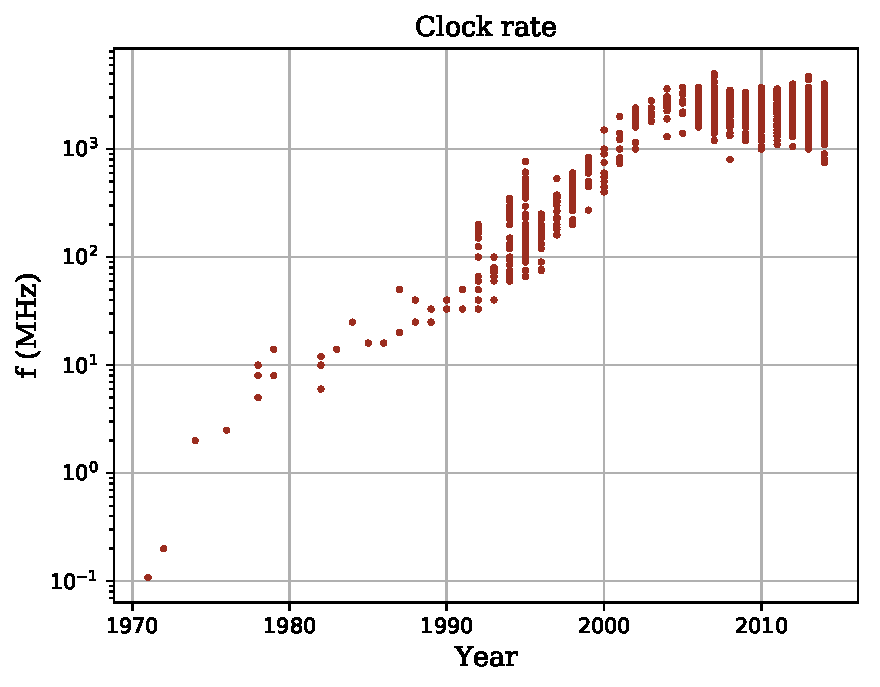
\includegraphics[width=\textwidth]{Source/ClockRate.pdf}
	\caption{Clock rate over the last 50 years. Drawn with data from \cite{cpudb}} %
	\label{fig-clockrate}
\end{figure}%
Figure \ref{fig-clockrate} shows how clock rate has changed over the last few decades. Up to about 2004, we see an exponential increase (note the logarithmic scale). This can mostly be attributed to shrinking feature size. If component size drops exponentially, and propagation speed stays constant then path delay drops exponentially. This means that frequencies can rise exponentially ($f=\frac{1}{T}$). \\
However, since the mid-noughties, clock rate has plateaued at around $\SI{3}{\GHz}$. This was not an anticipated stagnation. Even in 2005, textbooks still expected this exponential increase to continue. See for example \cite[p.~3]{lipastiShen}, where Lipasti and Shen wrote:
\begin{quote}
	\textit{By 2010, we can expect microprocessors to contain more than $1$ billion transistors with clocking frequencies greater than $\SI{10}{\GHz}$.}
\end{quote}
While the prediction about transistor count was quite accurate (the POWER7, released in 2010, for example, had around $\SI{1.2e9}{transistors}$ \cite[p.~44]{power7-2}), people still dream about $\SI{10}{\GHz}$ processors in 2019. To explain this plateau, we need to understand how power consumption in CMOS logic works.\\ 
\begin{figure} [h]
	\centering	
	\begin{minipage}{0.5\textwidth}
		\centering
		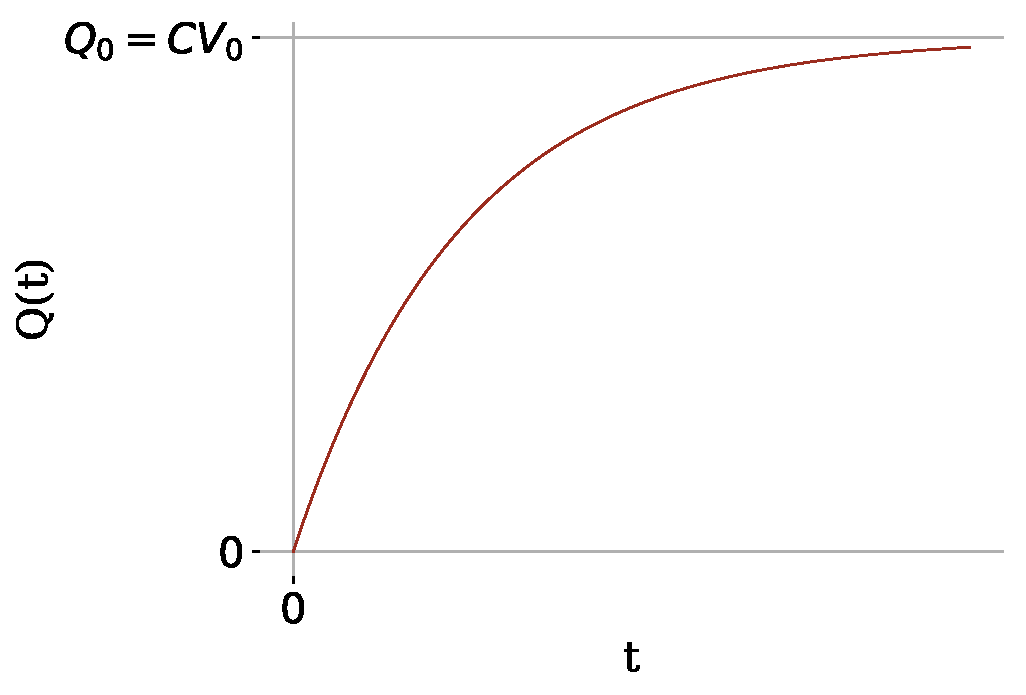
\includegraphics[width=\textwidth]{Source/Charging/charge.pdf}
	\end{minipage}%
	\begin{minipage}{0.5\textwidth}
		\centering
		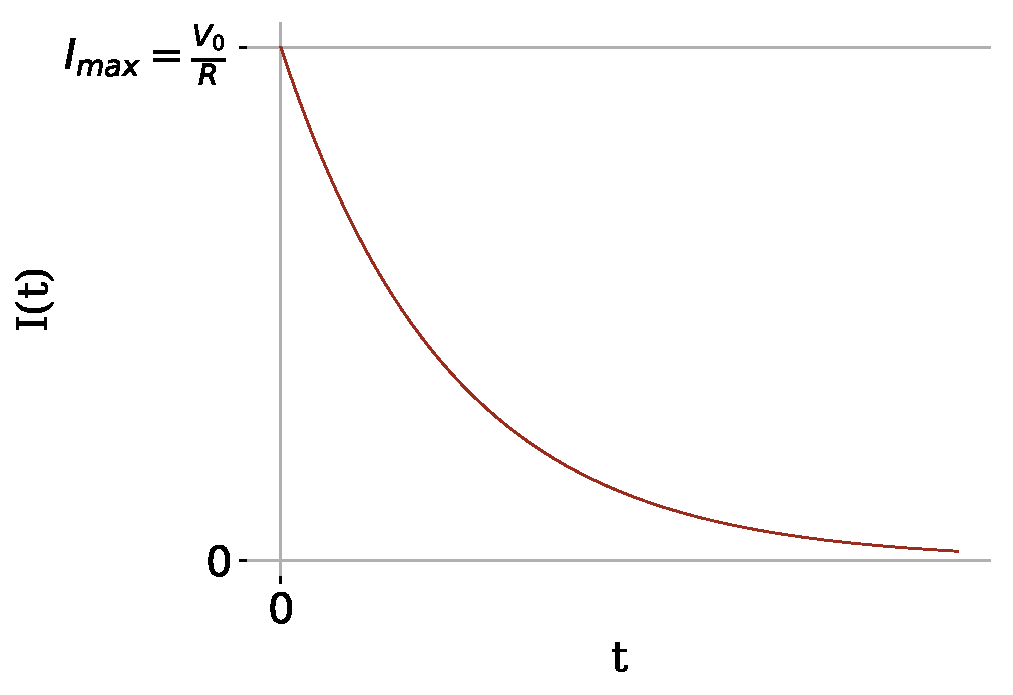
\includegraphics[width=\textwidth]{Source/Charging/current.pdf}
	\end{minipage}
	\caption{Charge and current for loading a capacitor over a resistor}%
	\label{fig-capacitorCharging}
\end{figure}%
The main source of power dissipation is dynamic switching power. Switching power is dissipated wherever parts of the circuitry are being charged/discharged. We can model this as a kind of capacitor which is charged over a resistor. The resistor corresponds to the resistance of all the wires and transistors. This is where power is dissipated in the form of heat. \\
We are now going to take a closer look at this charging process which is sketched in figure \ref{fig-capacitorCharging}. If we turn on the voltage source at $t=0$, the charge on the capacitor $Q(t)$ will start to rise to the full $Q_0 = CV_0$, where $V_0$ is the supply voltage and $C$ is the capacity of the capacitor. Figure \ref{fig-capacitorCharging} also shows the current which flows through the resistor. It is simply the derivative of the first curve $I(t)= \frac{d}{dt}Q(t)$. This current determines how much power is dissipated in the resistor.\\ 
Every charge transfer $dQ$ onto the capacitor comes with a transfer in energy, given by
\begin{equation}
	dE = VdQ
\end{equation}
Capacity $C$ is defined as charge $Q$ per voltage $V$ at any point in time, so we can write this as
\begin{equation}
	dE = \frac{Q}{C} dQ
\end{equation}
For a full charge to $Q_0$ we find\footnote{In practice, we will not reach that voltage, however the calculations are similar if we only require a charge of $\SI{0.95}{Q_0}$.}:
\begin{equation}
	\Delta E = \int_{0}^{Q_0} \frac{Q}{C} dQ = \frac{1}{2} \frac{Q_0^2}{C} = \frac{1}{2} C V_0^2 = \frac{1}{2} Q_0 V_0
\end{equation}
However, the voltage source supplies the full $Q_0 V_0$. So the other $\frac{1}{2}Q_0 V_0$ are dissipated in the resistance in the form of heat. If we also include the heat dissipated in the discharge, then the total energy lost per ``clock cycle'' is
\begin{equation}
	\frac{\Delta E}{cycle} = \alpha Q_0 V_0 = \alpha C V_0^2
\end{equation}
where I have included an activity factor $\alpha$. This accounts for the fact that not every transistor is switching every clock cycle.\\ 
Now, power is $P=\frac{\Delta E}{\Delta t}$ and frequency is $f=\frac{cycles}{\Delta t}$, so
\begin{equation}
	P = \frac{\Delta E}{\Delta t} = \frac{\Delta E}{cycle} \times \frac{cycles}{\Delta t} = \alpha CV_0^2f \label{eq-power}
\end{equation}
The capacitance of each transistor has historically scaled down with CMOS dimensions \cite{dennardScaling} but because of the increase in transistor numbers, we should expect the total capacitance to stay constant. \\
Equation \ref{eq-power} tells us that power dissipation scales quadratically with voltage. To keep power low, voltage needs to be kept low. Figure \ref{fig-vdd} shows that supply voltage has indeed decreased over the last two decades. The first plateau at $\SI{5}{\V}$ simply is due to convention before a decrease in power became necessary \cite{recordingCPUHistory}.
\begin{figure}[!h]
	\centering
	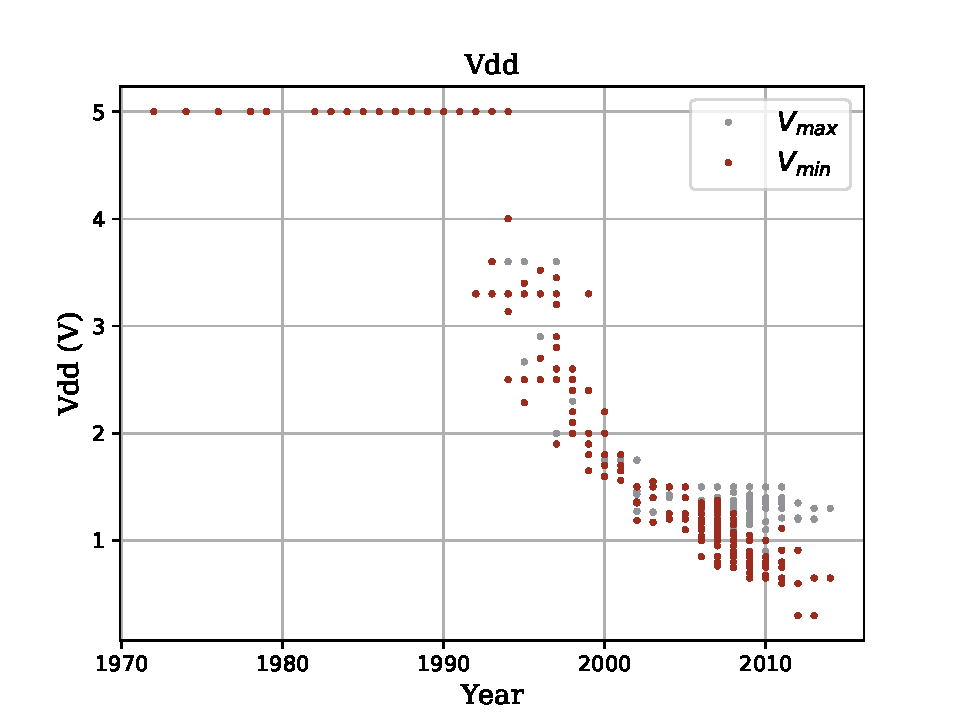
\includegraphics[width=\textwidth]{Source/Vdd.pdf}%
	\caption{$V_{dd}$ over the last 50 years. Drawn with data from \cite{cpudb}.}% %\note{The extremely low Vdd values are from \url{https://ark.intel.com/content/www/us/en/ark/products/70097/intel-atom-processor-z2480-512k-cache-up-to-2-00-ghz.html}}}%
	\label{fig-vdd}
\end{figure}%
The thermal voltage $\frac{kT}{e} \approx \SI{26}{\mV}$ (at $\SI{300}{\kelvin}$) gives an ultimate lower limit on the operating voltage \cite{designNearTheLimits}. Lower operating voltages also increase leakage currents \cite{ComputingsEnergyProblem} \cite{ScalingBelow1Mu}. This has resulted in $V_{dd}$ plateauing at around $\SI{1}{\volt}$ (with some manufacturers allowing for lower values in low-power modes). The change in voltage is, however, rather minor compared to the change in the order of magnitude of the clock frequency in figure \ref{fig-clockrate}. So we would expect power to scale very similarly to clock frequency, as $P\propto f$, according to equation \ref{eq-power}.%
\begin{figure}[!t]
	\centering
	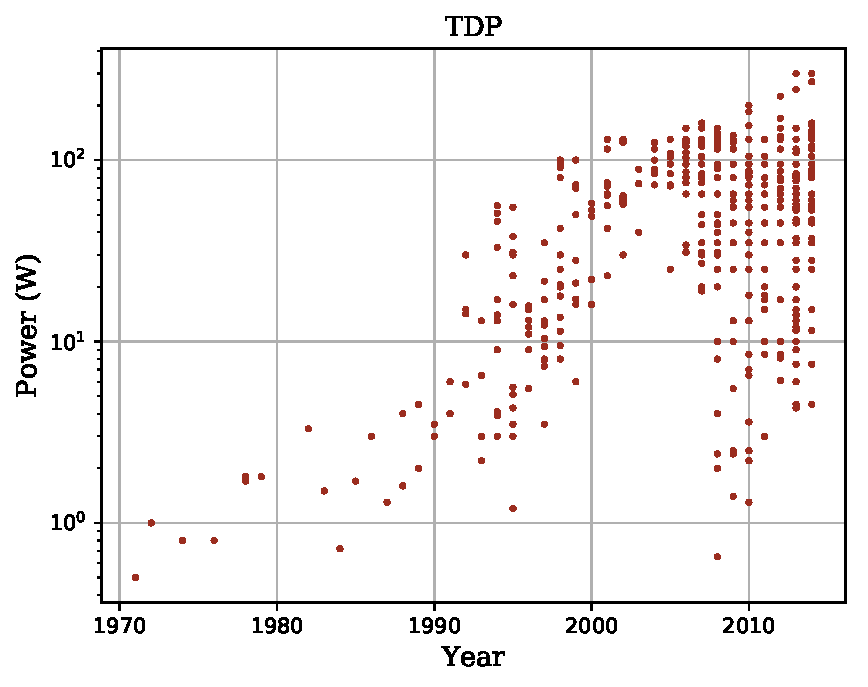
\includegraphics[width=\textwidth]{Source/TDP.pdf}
	\caption{TDP over the last 50 years. Drawn with data from \cite{cpudb}} 
	\label{fig-tdp}
\end{figure}%
And indeed, figure \ref{fig-tdp} shows that this is the case. It plots thermal design power which is the maximum amount of power that a processor is designed to dissipate. More power means that the system needs to have a more powerful cooling system. In \cite{ComputingsEnergyProblem}, Horowitz claims that the limit to air cooling for personal computers is around $\SI{100}{\watt}$. The data from the Stanford CPU DB seems to support that estimate. As figure \ref{fig-tdp} demonstrates, the upper limit for thermal design power (TDP) has stagnated and it did so at around the same time as clock rate (compare to figure \ref{fig-clockrate}). \\
Figure \ref{fig-tdp} also shows that since then, manufacturers have started offering a wide array of products from low-power to high-power devices. Many researchers argue that this trend in application-specific optimisation has allowed and will continue to allow scaling of performance even if CMOS scaling laws are coming to an end \cite{ComputingsEnergyProblem} \cite{ApplicationDependentScaling} \cite{MaintainingBenefitsWhenScalingBogsDown} \cite{PowerConstrainedCMOSScalingLimits}.\\

There are two other sources of power, short-circuit power and static power. Short-circuit power is dissipated every clock cycle when both nMOS and pMOS transistors are briefly on and there is a short circuit between $V_{dd}$ and $GND$. Static power is dissipated due to leakage currents in transistors. The latter is becoming a greater problem as transistors get smaller. But the similarity between the change in clock rate and the change in power suggests that it can be neglected in this discussion. \\

This estimation explains why we have seen a plateau in clock speed over the last decade. Higher clock speeds will require a more sophisticated cooling method or transistor design.\\


\textbf{Alternative approaches to computing}\\
These limits could also potentially be overcome by pursuing more exotic approaches to computing, like asynchronous or neuromorphic logic. However, the investment barrier might be too high for such radical changes. In \cite{ComputingsEnergyProblem} Horowitz states that he is ``sure there are better technologies out there'' but that we might be stuck with CMOS for computing because of two big reasons. Firstly, we have invested enormously in the physical manufacturing process of CMOS technologies and any competition would have to have a huge inherent advantage to compete with it. Secondly, CMOS VLSI has greatly influenced our design abstractions. A new technology would require a completely new design flow and new tools to compete. \\
Single-core performance is still rising, even though clock speeds have stagnated \cite{recordingCPUHistory}. But when it eventually reaches its limits and all inherent parallelism is exploited, other technologies might have a chance to shine. Until then, researchers looking into ideas like neuromorphic, asynchronous or quantum logic need to develop tools and design abstractions to make their technologies viable alternatives.


\newpage

\cleardoublepage

\phantomsection
\addcontentsline{toc}{section}{Assembly code in this thesis}
\label{sec-assembly}
\textbf{\Large Assembly code in this thesis}\\
 
This thesis occasionally contains assembly code snippets. I restricted myself to ADD and LD instructions from the RV64I Base Integer Instruction Set.\\
RISC-V is a load-store architecture, which means that memory is only accessed by load and store instructions that move data between registers and memory. Calculations can only be performed on registers. \\ 
A LD instruction  
\begin{assembly}
	\begin{tabularx} {\textwidth} {n o a a X}
		& LD 	& rd & imm(rs1) \\
	\end{tabularx}
\end{assembly}
loads a 64-bit value from memory and saves it in rd. The effective byte address is calculated by adding the immediate imm to the content of rs1.\\
An ADD instruction has the form
\begin{assembly}
	\begin{tabularx} {\textwidth} {n o a a X}
		& ADD 	& rd & rs1		& rs2 \\
	\end{tabularx}
\end{assembly}
where rs1, rs2 and rd are registers. It adds the contents of the source registers rs1 and rs2 and saves the result in the destination register rd.\\

\cite[p.~5, p.~18f, p.~31]{riscv}


\vspace{2cm}


\phantomsection
\addcontentsline{toc}{section}{About RISC-V}
\label{sec-riscv}
\textbf{\Large About RISC-V}\\

RISC-V is an open-source ISA. It was developed at the University of California, Berkeley for research and education purposes. RISC stands for reduced instruction set computer. The idea behind it is that few simple instructions are easier to work with than many complex instructions.\\
RISC-V gives researchers in academia the opportunity to study and develop actual hardware implementations without having to pay royalties for commercial ISAs. \\

\cite{RISCV-webpage} \cite[p.~1-3]{riscv}


\newpage

\cleardoublepage
\phantomsection
\addcontentsline{toc}{section}{\listfigurename}
\label{sec-lof}
\listoffigures

\newpage

\cleardoublepage
\phantomsection
\addcontentsline{toc}{section}{List of Acronyms}
\label{sec-loa}
{\textbf{\Large List of Acronyms}\\
	
	{
		\setlength{\extrarowheight}{10pt}
		\hfill \break
		\begin{tabularx} {\textwidth} {p{5cm} X}
			BOOM & Berkeley Out-of-Order Machine\\
			CMOS & Complementary metal-oxide-semiconductor\\
			cTDP & Configurable thermal design power\\ 
			DVFS & Dynamic voltage and frequency scaling\\
			ID   & Instruction decode (stage)\\
			II   & Instruction issue (stage)\\
			ILP  & Instruction level parallelism\\
			INT  & Integer (unit)\\
			IPC  & Instructions per cycle\\
			ISA  & Instruction set architecture\\
			LS	 & Load-store (unit)\\
			PC	 & Program counter\\
			RAT  & Register alias table\\ 	
			RF	 & Register file\\        
			RISC & Reduced instruction set computer\\
			ROB  & Reorder buffer\\     
			RS	 & Reservation station\\  
			RTL	 & Register-transfer level\\ 
			SMT	 & Simultaneous multithreading\\
			TDP	 & Thermal design power\\	
			VLIW & Very long instruction word (architecture)\\
			
		\end{tabularx}
		\hfill \break
		\newpage
	}


\newpage 
\thispagestyle{empty}
\begin{thebibliography}{56} % APA citation style      
    
    \bibitem{lipastiShen} 
    Shen, J. P., \& Lipasti, M. H. (2013). \textit{Modern processor design: fundamentals of superscalar processors}. Waveland Press.   
    
    \bibitem{Hennessy} 
    Hennessy, J. L., \& Patterson, D. A. (2011). \textit{Computer architecture: a quantitative approach}. Elsevier.
        
    \bibitem{tomasulo} 
    Tomasulo, R. M. (1967). An efficient algorithm for exploiting multiple arithmetic units. \textit{IBM Journal of research and Development, 11(1)}, 25-33.
    
    \bibitem{ProcessorArchitecture} 
    Silc, J., Robic, B., \& Ungerer, T. (2012). \textit{Processor architecture: from dataflow to superscalar and beyond}. Springer Science \& Business Media.
    
    \bibitem{power1}
    Oehler, R. R., \& Blasgen, M. W. (1991). IBM RISC System/6000: Architecture and performance. \textit{IEEE Micro, 11(3)}, 14-17.
    
    \bibitem{top500}
    TOP500 reports. Retrieved from \url{top500.org} on 08.06.2019.
    
    \bibitem{power2}
    White, S. W., \& Dhawan, S. (1994). POWER2: Next generation of the RISC System/6000 family. \textit{IBM Journal of Research and Development, 38(5)}, 493-502.
    
    \bibitem{power3}
    O'Connell, F. P., \& White, S. W. (2000). Power3: The next generation of PowerPC processors. \textit{IBM Journal of Research and Development, 44(6)}, 873-884.
    
    \bibitem{power4}
    Tendler, J. M., Dodson, J. S., Fields, J. S., Le, H., \& Sinharoy, B. (2002). POWER4 system microarchitecture. \textit{IBM Journal of Research and Development, 46(1)}, 5-25.
    
    \bibitem{power5}
    Kalla, R., Sinharoy, B., \& Tendler, J. M. (2004). IBM Power5 chip: A dual-core multithreaded processor. \textit{IEEE micro, (2)}, 40-47.
    
    \bibitem{power6}
    Le, H. Q., Starke, W. J., Fields, J. S., O'Connell, F. P., Nguyen, D. Q., Ronchetti, B. J., ... \& Vaden, M. T. (2007). Ibm power6 microarchitecture. \textit{IBM Journal of Research and Development, 51(6)}, 639-662.
    
    \bibitem{power7}
    Sinharoy, B., Kalla, R., Starke, W. J., Le, H. Q., Cargnoni, R., Van Norstrand, J. A., ... \& Nguyen, D. Q. (2011). IBM POWER7 multicore server processor. \textit{IBM Journal of Research and Development, 55(3)}, 1:1-1:8.
    
    \bibitem{power8}
    Sinharoy, B., Van Norstrand, J. A., Eickemeyer, R. J., Le, H. Q., Leenstra, J., Nguyen, D. Q., ... \& Levitan, D. (2015). IBM POWER8 processor core microarchitecture. \textit{IBM Journal of Research and Development, 59(1)}, 2:1-2:21.
    
    \bibitem{power9}
    Sadasivam, S. K., Thompto, B. W., Kalla, R., \& Starke, W. J. (2017). IBM Power9 processor architecture. \textit{IEEE Micro, 37(2)}, 40-51.
    
    \bibitem{intelSM}
    Intel Corporation. (2011). \textit{Intel® 64 and IA-32 Architectures Software Developer’s Manual}. Volume 1. Order Number: 253665-039US. 
        
    \bibitem{amdSM}
    Advanced Micro Devices (2017). \textit{Software Optimization Guide for
    	AMD Family 17h Processors}. Revision 3.00. Publication No. 55723.
    
    \bibitem{riscv} 
    Waterman, A. \& Asanovic, K. (2017). \textit{The RISC-V Instruction Set Manual, Volme I: User-Level ISA}. Document Version 2.2. 
    
    \bibitem{surveyOfRF} 
    Mittal, S. (2017). \textit{A survey of techniques for designing and managing CPU register file. Concurrency and Computation: Practice and Experience}, 29(4), e3906. 
    
    \bibitem{meltdown}
    Lipp, M., Schwarz, M., Gruss, D., Prescher, T., Haas, W., Mangard, S., ... \& Hamburg, M. (2018). Meltdown. \textit{arXiv preprint arXiv:1801.01207}.
    
    \bibitem{spectre}
    Kocher, P., Genkin, D., Gruss, D., Haas, W., Hamburg, M., Lipp, M., ... \& Yarom, Y. (2018). Spectre attacks: Exploiting speculative execution. \textit{arXiv preprint arXiv:1801.01203}.
        
    \bibitem{valuePrediction}
    Fu, C. Y., Jennings, M. D., Larin, S. Y., \& Conte, T. M. (1998). Value speculation scheduling for high performance processors. \textit{ACM SIGOPS Operating Systems Review}, 32(5), 262-271.
    
    \bibitem{virtualRR}
    Sharafeddine, M., Akkary, H., \& Carmean, D. (2013, February). Virtual register renaming. In \textit{International Conference on Architecture of Computing Systems} (pp. 86-97). Springer, Berlin, Heidelberg.
    
    \bibitem{boom} 
   	Celio, C., Zhao, J., Gonzalez, A., \& Korpan, B. (2019). RISCV-BOOM Documentation.
    
    \bibitem{cpudb}
    Stanford VLSI Group. CPU DB. Retrieved from \url{cpudb.stanford.edu} on 20.04.2019.
    
    \bibitem{intelDataSheet} 
    Intel Corporation. (2019). \textit{8th and 9th Generation Intel® Core™ Processor Families Datasheet}. Volume 1 of 2, Revision 003. 
    
    \bibitem{caseAgainstACP}
    Huck, S. (2011). \textit{Measuring Processor Power. TDP vs. ACP}. Revision 1.1. Available at \url{intel.com/content/dam/doc/white-paper/resources-xeon-measuring-processor-power-paper.pdf}
    
    \bibitem{power7-2}
    Anselmi, G., Blanchard, B., Cho, Y., Hales, C. \& Quezada, M. (2010). \textit{IBM Power 770 and 780 Technical Overview and Introduction}. Available at \url{www.redbooks.ibm.com/redpapers/pdfs/redp4639.pdf}
    
    \bibitem{dennardScaling}
    Dennard, R. H., Gaensslen, F. H., Rideout, V. L., Bassous, E., \& LeBlanc, A. R. (1974). Design of ion-implanted MOSFET's with very small physical dimensions.\textit{ IEEE Journal of Solid-State Circuits, 9(5)}, 256-268.
    
    \bibitem{recordingCPUHistory}
    Danowitz, A., Kelley, K., Mao, J., Stevenson, J. P., \& Horowitz, M. (2012). CPU DB: recording microprocessor history. \textit{Communications of the ACM, 55(4)}, 55-63.
    
    \bibitem{designNearTheLimits} 
    Taur, Y. (2002). CMOS design near the limit of scaling. \textit{IBM Journal of Research and Development, 46(2.3)}, 213-222.
    
    \bibitem{ComputingsEnergyProblem}
    Horowitz, M. (2014, February). Computing's energy problem (and what we can do about it). In \textit{2014 IEEE international solid-state circuits conference digest of technical papers (ISSCC)} (pp. 10-14). IEEE.
    
    \bibitem{ScalingBelow1Mu}  
    Taur, Y., \& Nowak, E. J. (1997, December). CMOS devices below $0.1\mu m$: how high will performance go?. In \textit{International Electron Devices Meeting. IEDM Technical Digest }(pp. 215-218). IEEE.
    
    \bibitem{ApplicationDependentScaling} 
    Frank, D. J., Dennard, R. H., Nowak, E., Solomon, P. M., Taur, Y., \& Wong, H. S. P. (2001). Device scaling limits of Si MOSFETs and their application dependencies. \textit{Proceedings of the IEEE, 89(3)}, 259-288.
    
    \bibitem{MaintainingBenefitsWhenScalingBogsDown}
    Nowak, E. J. (2002). Maintaining the benefits of CMOS scaling when scaling bogs down. \textit{IBM Journal of Research and Development, 46(2.3)}, 169-180.
    
    \bibitem{PowerConstrainedCMOSScalingLimits}
    Frank, D. J. (2002). Power-constrained CMOS scaling limits. \textit{IBM Journal of Research and Development, 46(2.3)}, 235-244.
    
    \bibitem{RISCV-webpage}
    Webpage of the RISC-V Foundation. Retrieved from \url{riscv.org/risc-v-foundation} on 05.06.2019.
   
\end{thebibliography}

%TODO add empty page, so that ERKLÄRUNG is on the right
\newpage
\thispagestyle{empty}

\textbf{Erklärung}\\

Ich versichere, dass ich diese Arbeit selbstständig verfasst und keine anderen als die angegebenen Quellen und Hilfsmittel benutzt habe.\\

Heidelberg, den 10.06.2019\\ %TODO

\vspace{2cm}
Amanda Matthes

\end{document}